% =====================================================================
%  Journal extension of "Evaluation as Supervision" -- target: Journal of
%  Systems and Software (Elsevier), regular paper. Author's venue decision,
%  2026-10-08 (docs/paper/JOURNAL_PAPER_PLAN.md section 1).
%
%  Build:   latexmk -pdf main.tex        (from docs/paper/journal/)
%
%  Every number in this paper comes from docs/paper/RESULTS.md or from the
%  committed analysis outputs it names (backend/out_study/*/analysis.json,
%  backend/out_study/secondary_extra.json). The design and every deviation
%  from it come from docs/paper/PREREGISTRATION.md (frozen at the annotated
%  tag prereg-freeze; amendments section 0.1 A1-A9).
%
%  Placeholders:  \CSEVEN{...}  second-model (C7) material, pending the run
%                 \TODO{...}    open author decisions and pre-submission items
%  grep for both before submission; README.md lists them.
%
%  Do NOT edit ../main.tex -- that is conference paper #1, under review.
% =====================================================================
\documentclass[preprint,12pt,authoryear]{elsarticle}

\usepackage[T1]{fontenc}
\usepackage[utf8]{inputenc}
\usepackage{lmodern}
\usepackage{amsmath,amssymb}
\usepackage{graphicx}
\usepackage{booktabs}
\usepackage{array}
\usepackage{tabularx}
\usepackage{multirow}
\usepackage[section]{placeins}   % keep floats inside their own section
\usepackage{xcolor}
\usepackage{microtype}
\usepackage{enumitem}
\usepackage{tikz}
\usetikzlibrary{arrows.meta,positioning,fit,calc,backgrounds,shapes.misc}
\usepackage{pgfplots}
\pgfplotsset{compat=1.18}
\usepackage{lineno}
\usepackage[hidelinks,breaklinks]{hyperref}

% =====================================================================
%  Macros for the journal draft.
% =====================================================================

% ---- Draft placeholders ---------------------------------------------
% \CSEVEN{...}  material that waits on the second-model run (C7, plan D5b,
%               prereg amendment A10). Renders as an orange bracketed note.
% \TODO{...}    an open author decision or a pre-submission task. Renders as
%               a magenta bracketed note.
% Switch \showplaceholdersfalse to hide both (for a word count only -- never
% for submission: every placeholder must be resolved, not hidden).
\newif\ifshowplaceholders
\showplaceholderstrue
\definecolor{cseven}{RGB}{196,98,0}
\definecolor{todo}{RGB}{176,0,112}
\newcommand{\CSEVEN}[1]{\ifshowplaceholders{\color{cseven}\textsf{\small[C7:~#1]}}\fi}
\newcommand{\TODO}[1]{\ifshowplaceholders{\color{todo}\textsf{\small[TODO:~#1]}}\fi}
% A placeholder table cell or number: \CSEVENNUM{} prints a bold dash.
\newcommand{\CSEVENNUM}{\ifshowplaceholders{\color{cseven}\textbf{--}}\fi}

% ---- Notation ---------------------------------------------------------
\newcommand{\arm}[1]{\textsf{#1}}          % arms A0--A3, placements P0--P3
\newcommand{\op}[1]{\textsf{#1}}           % operators O1--O8
\newcommand{\verdict}[1]{\texttt{#1}}      % supervisor verdicts
\newcommand{\cls}[1]{\textit{#1}}          % outcome classes
\newcommand{\code}[1]{\texttt{#1}}
\newcommand{\pp}{\,pp}
\newcommand{\ci}[2]{[$#1$,\,$#2$]}         % a 95% interval; math mode turns
                                           % "-2.9" into a true minus sign
\newcommand{\model}{\texttt{gemini-2.5-flash}}

% ---- Layout -----------------------------------------------------------
\newcolumntype{L}[1]{>{\raggedright\arraybackslash}p{#1}}
\newcolumntype{R}[1]{>{\raggedleft\arraybackslash}p{#1}}
\newcolumntype{Y}{>{\raggedright\arraybackslash}X}   % tabularx, ragged
\setlist{itemsep=2pt,topsep=4pt}

% Verbatim prompt wording (arms, placements, C1): monospace cannot hyphenate,
% so set it small and ragged-right to keep long lines inside the text block.
\newenvironment{prompttext}%
  {\begin{quote}\footnotesize\ttfamily\raggedright}%
  {\end{quote}}

% Float placement: the preprint layout's text block is narrow (390pt) and
% tall tables otherwise drift to the end of the document.
\renewcommand{\topfraction}{0.9}
\renewcommand{\bottomfraction}{0.8}
\renewcommand{\textfraction}{0.07}
\renewcommand{\floatpagefraction}{0.75}
\setcounter{topnumber}{3}
\setcounter{bottomnumber}{2}
\setcounter{totalnumber}{5}


\journal{Journal of Systems and Software}

\begin{document}

\begin{frontmatter}

% Working title; alternative kept for the author's choice:
%   "Evaluation as Supervision, Revisited: Repair, Propagation and the Limits
%    of Local Verification in a Multi-Agent LLM Pipeline"
\title{Does Measured Feedback Repair Defects in LLM Pipelines?\\
A Pre-registered Fault-Injection Study of Deterministic Runtime Supervision}

% ---------------------------------------------------------------------
% TODO (D5, JOURNAL_PAPER_PLAN section 2 item 1): the journal author list is
% an open author decision. The block below is the conference #1 list, kept as
% the default until the author decides. JSS: single-anonymised review, so
% names appear in the submission. The corresponding author's affiliation
% alone decides CAUL open-access eligibility (APC waived for a Swinburne
% University of Technology affiliation, institutional email required).
% ---------------------------------------------------------------------
\author[swin]{Huu Hoan Hoang\corref{cor1}}
\ead{105732188@student.swin.edu.au}
\author[swin]{Ho Quang Dung Pham}
\author[swin]{Manh Duc Tran}
\author[swin]{Nam Khanh Nguyen}
\author[swin]{Manh Toan Nguyen}
\cortext[cor1]{Corresponding author.}
\affiliation[swin]{organization={Swinburne Vietnam, FPT University},
                   city={Hanoi},
                   country={Vietnam}}

\begin{abstract}
A deterministic supervisor can check outputs in a large language model (LLM)
pipeline and retry a stage with measured feedback. We evaluate whether the
feedback content repairs defects in a pre-registered fault-injection study of a
four-stage review-analysis pipeline. Six operators produced 142 defects over 28
workloads; the confirmatory core comprised 1,167 trials. Measured facts repaired
94.7\% of defects and a contentless rejection 94.0\% (+0.7 percentage points,
95\% CI $-2.9$ to +4.3; exact McNemar $p=0.754$). In an exploratory analysis,
measured facts increased unconditional exact restoration to the clean output by
14.6 points (68.1\% vs 53.5\%, 95\% CI +8.2 to +21.3). At the reasoning stage, restored outputs were
associated with less downstream report divergence than repaired rewrites;
these post-treatment subgroups do not establish causation. A zero thinking-token
budget retained high repair but some trials needed schema retries. A small local
model showed an exploratory +6.8-point repair contrast, with sensitivity to
repetition and model/runtime differences. Production retry was accepted on
28.2\% of real defects versus 98.5\% of injected defects; acceptance is not
correctness. Showing the defective artifact reduced measured collateral damage
from 38.4\% to 1.1\% in the placement cell. These results distinguish local
repair, restoration, verifier acceptance and downstream preservation.

\end{abstract}

\begin{keyword}
large language models \sep
runtime verification \sep
fault injection \sep
self-correction \sep
multi-agent systems \sep
pre-registration
\end{keyword}

\end{frontmatter}

\TODO{Draft of 2026-10-08. Open before submission: author list and
corresponding author (D5); the conference-version declaration and its timing
(Section~\ref{sec:intro-extension}); data availability; the Tier-C citations
marked in Section~\ref{sec:related}; the generative-AI declaration; and every
\textsf{[C7]} placeholder, which waits on the second-model run.}

\linenumbers

% =====================================================================
\section{Introduction}
\label{sec:intro}
% =====================================================================

Large language models (LLMs) are increasingly composed into multi-stage
pipelines in which each stage is an agent with a typed output contract, and
those pipelines are shipped as software components. Structured-output tooling
has made the components reliably \emph{well-formed}, but well-formed is not
grounded. An evidence identifier can be syntactically perfect and point at
nothing. A recommendation can validate against its schema and have no
connection to anything an earlier stage found. A report can restate content
that no stage produced. Each of these passes every check the type system
offers. Catching such defects while the pipeline runs, and doing something
about them, is a verification problem in the ordinary software-engineering
sense: a component's output must be checked against a specification that its
types do not capture~\citep{leucker2009rv}.

In the conference version of this work~\citep{hoang2026eas}, we built such a
check into a four-stage pipeline that analyses restaurant reviews. Every stage
reads only what earlier stages produced in the same run, so every claim a stage
makes can be checked against upstream state alone. A deterministic supervisor
measures each stage's output, decides by fixed rules whether to proceed, warn,
retry or halt, and on a retry writes the measured failure into the prompt of
the stage being re-run. It makes no model call of its own. That study measured
how often an unsupervised pipeline emits ungrounded content. It could not
measure whether the retry \emph{repairs} it: its enforcing arm produced a single
retry. Repair is the property that determines whether such a supervisor is
worth building, because a runtime check that detects defects but cannot get
them fixed only halts the pipeline.

Whether measured feedback repairs is genuinely contested, and the two relevant
literatures disagree in a way an experiment can settle. One holds that feedback
\emph{content} is the active ingredient. In code repair, better feedback
produces better repairs. On 40 failing programs, human-written explanations
raised the share of successful repairs from 33.3\% to 52.6\% over model-written
ones~\citep{olausson2024selfrepair}. Models that cannot find their own reasoning
errors can correct many of them once the location is
supplied~\citep{tyen2024}. The other holds
that the \emph{signal} that something is wrong does most of the work. A bare
continuation cue closes most of the gap between how models correct others'
errors and their own~\citep{tsui2026scbench}. In self-debugging, the least
informative feedback condition recovers much of the gain of the most
informative one when execution still decides whether a revision is
needed~\citep{chen2024selfdebug}. A deterministic supervisor's feedback sits at
the informative extreme. It names the offending item and the measured fact.
If content binds, measured-fact feedback should repair more defects than a
rejection that says nothing. If the signal is what matters, the two should
repair alike.

We test this in a pre-registered fault-injection study. Six operators corrupt
clean stage outputs taken from 28 real pipeline runs, giving 142 defects, each
designed to trip exactly one supervisor check. Each defective stage is re-run
through its production agent under four arms: the production measured-fact
feedback; the same message with the facts removed; the defect presented as a
fresh correction task, which serves as a capability ceiling; and a bare
regeneration. The single confirmatory test, fixed with the arm wording, the
outcome coding and the analysis before any trial ran, compares the first two.
Around the confirmatory core of 1{,}167 trials, exploratory cells vary
where the defective output appears, the sampling temperature, the extent of
the defect, whether the stage's obligations are restated, and the reasoning
budget allocated to internal thinking traces. Table~\ref{tab:cells} distinguishes trials from downstream conditions and calls. They also replay 13 real defects that the production
supervisor caught, follow every defect into the later stages, and measure what
the supervisor's deterministic overwrite of one statistic buys over a retry.
Another repeats the core's arms on a second, open-weight model served locally.

The confirmatory contrast found little difference in overall repair on the
hosted model near its ceiling. Exploratory analyses found that measured facts
increased unconditional exact restoration to the clean output, and that
restoration outcomes were associated with downstream divergence. These
post-treatment associations do not establish a causal mechanism. The local
model showed lower repair and an exploratory feedback advantage. The production
retry was accepted much less often on real defects than on injected ones, many
of which were judged differently by blinded raters.

The contributions are a pre-registered, gated fault-injection protocol and
paired feedback-content comparison; evidence on exact restoration and its
qualified downstream association; a real-defect replay and second-model
comparison; and calibration and propagation analyses that expose limits of
stage-local verification. Section~\ref{sec:design-rq} states RQ1--RQ6.

\paragraph{Relation to the conference version}
\label{sec:intro-extension}
This article extends the conference paper accepted at EAI FISAT
2026~\citep{hoang2026eas}, which introduced the supervisor, the derivability
property and the measurements of defect incidence and instability.
Section~\ref{sec:system} summarises that system in new text. Everything from
Section~\ref{sec:design} onwards is new: the pre-registered repair study, every
trial, the real-defect replay, the downstream-propagation analysis and the
calibration. Section~\ref{sec:discussion-reconcile} lists the points at which
the new results revise claims made in the conference version.

The rest of the paper is organised as follows. Section~\ref{sec:related}
positions the study. Section~\ref{sec:system} describes the system and
Section~\ref{sec:design} the study design. Section~\ref{sec:results} reports
the results by research question. Section~\ref{sec:discussion} discusses what
they mean for building runtime supervisors, Section~\ref{sec:threats} the
threats to validity, and Section~\ref{sec:conclusion} concludes.

% =====================================================================
\section{Background and related work}
\label{sec:related}
% Facts about cited papers come from the reading-list extractions in
% ../Reading List/Tier_A/Tier_A_extraction.md and Tier_B/*.md, which were
% read against the PDFs. Every number quoted here carries the denominator or
% caveat those extractions flag. The Tier-C papers (JOURNAL_PLAN section 2)
% were read in full on 2026-10-20 before they were cited: AgentSpec and
% Reddy et al. (Section 2.1), AgenTracer and Who&When (Section 2.3), and
% Defects4J (Section 2.4).
% =====================================================================

\subsection{Verifying LLM pipeline outputs at run time}
\label{sec:related-rv}

Runtime verification checks behaviour against a specification during
execution~\citep{leucker2009rv}. Multi-agent frameworks divide tasks among
specialised agents \citep{metagpt,camel,chatdev,autogen}; coordination remains
an open problem~\citep{guo2024survey}. Output schemas do not establish that a
stage's claims are grounded in its inputs. LLM judges \citep{geval,mtbench}
can assess outputs but exhibit position and self-preference biases
\citep{positionbias,selfpreference}. External-tool feedback can improve
correction but needs a trusted resource~\citep{critic}. Our deterministic
checks use pipeline state and detect missing provenance, not falsity
\citep{hoang2026eas}. They also identify the check class and location by
construction, a difficult post-hoc diagnosis problem
\citep{tan2026agentchaos}.

AgentSpec enforces event-triggered policies~\citep{wang2026agentspec};
\citet{reddy2026gates} use deterministic gates before an airline agent's tool
calls, raising task success from 29.6\% to 42.0\% with gpt-4o-mini. Those
systems check actions against policies. Our supervisor checks stage outputs
against upstream state, and compares informative and generic rejections.

\subsection{Self-correction and the role of feedback}
\label{sec:related-selfcorrection}

A large literature studies whether a model can improve an output when told,
or when it tells itself, that the output is wrong. In Self-Refine the model
critiques and revises its own output~\citep{selfrefine}, and Reflexion carries a
verbal reflection on failure into later attempts~\citep{reflexion}. In their
survey of these methods, \citet{pan2024survey} observe that when a model
produces its own feedback, the quality of that feedback is constrained by the
model's limitations, and that recent work therefore draws feedback from external
tools such as trained models, code interpreters and search engines.
Two critical studies narrow the claim. \citet{huang2024cannot} show that,
without an oracle deciding when to stop, intrinsic self-correction does not
improve reasoning and often degrades it. They also caution that feedback
messages can carry task information the original prompt omitted, which makes a
feedback effect partly a prompt-completeness effect. \citet{kamoi2024} classify
correction driven by an external, non-LLM verifier as a fair setting distinct
from intrinsic self-correction. They identify feedback generation as the
bottleneck and recommend measuring feedback quality directly. Our supervisor is
such an external verifier. Its feedback is generated deterministically and is
correct by construction about what it measures.

Whether feedback \emph{content} matters, as distinct from the signal that a
revision is needed, is where the literature divides. \citet{olausson2024selfrepair}
establish two norms for repair claims. A repair must be compared with
independent resampling at an equal budget. And feedback quality is binding:
substituting human-written for model-written explanations raised successful
repairs from 33.3\% to 52.6\%, on a deliberately easy sample of 40 failing
programs. \citet{tyen2024} separate finding an error from correcting it. Models
locate the first error in a reasoning trace poorly, but given its location, a
simple backtracking procedure corrected 18 to 44 percentage points of
previously incorrect traces, and supplying a random location roughly halved
the gain. In self-debugging, \citet{chen2024selfdebug} find that their least
informative feedback condition retains much of the benefit of the most
informative ones, because execution still decides whether to revise. Removing
that trigger can push accuracy below the no-repair baseline. Two studies
manipulate presentation rather than content. \citet{tsui2026scbench} injects the
same error either into the user's turn or into the model's own, and finds that
models correct the external error far more often. Its self-correction blind
spot, one minus the ratio of the internal to the external correction rate,
averages 64.5\% across 14 models. Appending a contentless continuation cue
(``Wait'') reduces that blind spot by 89.3\%. \citet{chen2026rolerelabel}, in
an unrefereed preprint, hold an erroneous claim byte-identical while changing
only the chat role that carries it. Explicit correction rises by 23 to 93
points, significantly in 10 of 12
model--domain combinations. Two code-repair studies shape the single-retry
design: a second editing round can degrade results~\citep{zhang2023selfedit}, and
most of the gain from iterated repair arrives in the first round or
two~\citep{arimbur2026}. \citet{arimbur2026} also documents run-to-run variation
in greedy decoding on hosted inference APIs, a threat this study measures
directly.

None of these studies holds the defect fixed and varies only what the failing
stage is told, under a deterministic external checker, with the placement of
the defective output controlled. Arms \arm{A1} and \arm{A2} of our design are
exactly that manipulation. Our placement factor reproduces the user-turn versus
own-turn contrast of \citet{tsui2026scbench} and \citet{chen2026rolerelabel},
and adds the placement that production retries actually use, in which the
defective output is absent.

\subsection{Fault injection and failure analysis in multi-agent LLM systems}
\label{sec:related-fi}

Injecting faults to observe how a system degrades has a long engineering
lineage, including chaos engineering of production services~\citep{basiri2016chaos}.
Its recent application to LLM agents has developed along two tracks.
\emph{Failure analysis} catalogues what goes wrong. \citet{cemri2025mast}
derive a taxonomy of 14 failure modes in three categories from expert annotation
of multi-agent traces, with inadequate task verification as one of the three
principal categories. They observe that verifiers often perform only
superficial checks, and that the presence of a failure mode is only loosely
coupled with whether the task succeeds. \emph{Fault injection} measures how
damage propagates. \citet{huang2025resilience} corrupt agents' profiles or
messages and find that linear structures degrade most and hierarchical ones
least. Corrupting a profile also degrades performance more than corrupting
messages, so the two injection methods are not interchangeable.
MAS-FIRE~\citep{jia2026masfire}, a preprint, injects 15 types of fault through
prompts, intercepted outputs and message routing. It separates whether a system
detects a fault, whether it resolves it locally, and whether the task still
succeeds. AgentChaos~\citep{tan2026agentchaos} injects 65 configurations of
crash, omission and value faults at the boundary between agent and LLM API.
It discards tasks in which the configured fault never fired, a trigger
verification our design adopts. It finds that injection position matters most
for pipeline architectures, and that silent failures, plausible outputs with no
warning, account for 22\% to 66\% of failures depending on the system.
A third line of work, failure attribution, asks which agent and which step
caused a failed run. Who\&When~\citep{zhang2025whowhen} is a benchmark of
hand-annotated failure logs from 127 multi-agent systems; the best of the three
attribution methods evaluated on it found the decisive step in 14.2\% of cases.
AgenTracer~\citep{zhang2026agentracer} labels runs automatically to train an
attribution model. Failed runs are labelled by counterfactual replay, which
corrects one action at a time and re-runs the rest; successful runs become
failures through an injected fault, whose step is then known by construction.
Attribution locates a fault after a run has failed. Our supervisor locates a
defect while the pipeline runs, and our injections measure whether the retry
then removes it.

This work measures tolerance, propagation and diagnosis. None of it measures
whether a supervisor's feedback gets a defect \emph{repaired}. None of it checks
whether the injected faults behave like the faults the system produces on its
own.

\subsection{Synthetic faults as proxies for real ones}
\label{sec:related-proxy}

Software engineering asked the second question of mutation analysis long
before LLM pipelines existed. Testing studies commonly used hand-seeded faults
and mutants in place of real bugs, which are hard to extract and reproduce.
Defects4J~\citep{just2014defects4j} was built to make real faults available
for controlled studies. \citet{just2014mutants} test whether artificial
mutants can stand in for real faults. Across 357 real faults in five Java
programs, 73\% were coupled to mutants from commonly used operators, and a
test suite's mutant detection correlated with its real-fault detection beyond
what coverage explains. Their coupling concerns \emph{detection}. They note that
it is unclear whether fault-localisation and program-repair techniques
evaluated on mutants perform equally well on real faults. Our design faces the
same question for repair: whether a repair rate measured on injected defects
says anything about the defects a pipeline produces. We answer it empirically.
The 13 defects the production supervisor caught are replayed through the same
retry. Before the study, blinded raters compared real and injected defects, and
both results are reported beside the injected-defect rates
(Sections~\ref{sec:design-operators} and~\ref{sec:results-rq3}).

% =====================================================================
\section{The system under study}
\label{sec:system}
% Condensed from the conference version (hoang2026eas), rewritten rather than
% reused. Code: backend/app/core/supervision.py, graph.py; agents in
% backend/app/agents/. Do not copy prose from ../main.tex.
% =====================================================================

The system is the review-analysis pipeline and runtime supervisor of the
conference version of this work~\citep{hoang2026eas}. We describe here only what
the study manipulates or measures. Neither the pipeline nor the supervisor was
changed for the study.

\subsection{A staged pipeline}
\label{sec:system-pipeline}

The pipeline analyses the reviews of one business in four stages. Each stage is
an LLM agent whose output must validate against a typed contract.
\emph{Analysis} reads the raw reviews and labels each one with an overall
sentiment and a set of aspects drawn from a fixed seven-category taxonomy,
each with its own polarity. \emph{Reasoning} groups these labels into
\emph{patterns}, each consisting of an aspect, a description, a frequency and
a non-empty list of review identifiers cited as evidence. It also proposes
\emph{root causes} that link a pattern to an explanation. \emph{Strategy} turns
patterns and root causes into prioritised recommendations, each consisting of
an issue, an action and an expected impact. \emph{Report} composes the
document a user reads. It restates root causes and recommendations, together
with the business's name and the sample size, which the pipeline supplies as
trusted values.

The pipeline is \emph{closed}. Apart from analysis, which alone reads the raw
reviews, every stage reads only outputs that earlier stages produced in the
same run. No stage has a scratchpad, a retrieval call, a tool or a memory of
earlier runs. Closure gives every claim a checkable provenance. A claim in a
stage's output either derives from upstream outputs or was introduced by that
stage, because information has no other way in. Groundedness is therefore
decidable by consistency checking against upstream state, with no labels and no
second model. We call this the \emph{derivability} property. It licenses
detecting the absence of provenance, not falsity: an output can be faithfully
derived from an upstream error.

\subsection{The supervisor: measure, then decide}
\label{sec:system-supervisor}

Control passes through a single orchestrator node after every stage. The
orchestrator calls two deterministic functions. \code{measure()} computes facts
about the stage's output relative to upstream state and applies no thresholds.
\code{decide()} maps those facts to one of four verdicts by fixed rules:
\verdict{proceed}, \verdict{proceed\_with\_warning}, \verdict{retry} or
\verdict{halt}. Table~\ref{tab:checks} lists the checks. The supervisor makes no
model call. Its verdicts are reproducible, cost nothing at the margin, and can
be recomputed offline from stored facts, which is what makes the replays and
re-scorings in this study possible.

\begin{table}[tbp]
\centering
\caption{The supervisor's checks at the three stages the study injects into.
Each check resolves against upstream state only. An analysis-stage check
(contradiction between a review's star rating and its predicted sentiment)
exists but is not exercised here.}
\label{tab:checks}
\footnotesize
\begin{tabularx}{\linewidth}{@{}l Y L{2.9cm} l@{}}
\toprule
Stage & Measured fact & Check class & Verdict \\
\midrule
Reasoning & a cited evidence identifier does not resolve to any analysed
  review & unresolvable evidence id & \verdict{retry} \\
 & a cited review does not mention the pattern's aspect & misaligned aspect &
  \verdict{retry} \\
 & the claimed frequency differs from the recomputed one by more than 0.05 &
  frequency divergence & warning \\
Strategy & a recommendation's issue has character-level similarity below
  0.35 to every upstream pattern and root cause & untraceable recommendation &
  \verdict{retry} \\
Report & a root cause or recommendation is absent from the upstream outputs &
  report containment & \verdict{retry} \\
 & the business name or sample size differs from the trusted values &
  trusted metadata & \verdict{retry} \\
\bottomrule
\end{tabularx}
\end{table}

A retry re-runs the stage. The retry cap is applied to the verdict, not inside
the checks. Once a stage has been retried twice, a further \verdict{retry}
becomes \verdict{halt} at the analysis, reasoning and report stages, and
\verdict{proceed\_with\_warning} at strategy, which is the one non-critical
stage. Each stage therefore runs at most three times, and the run's length is
bounded by the routing function rather than by the agents eventually
succeeding.

\subsection{Retry feedback}
\label{sec:system-feedback}

On a retry, the measured fact that triggered the verdict is written into the
re-run stage's prompt. The production template, which is arm \arm{A1} of this
study, reads in full:

\begin{prompttext}
A deterministic quality check rejected your previous answer to this task:\\[2pt]
\{feedback\}\\[2pt]
Produce a corrected answer that fixes exactly these issues. Return only valid
JSON.
\end{prompttext}

\noindent Here \code{\{feedback\}} is the supervisor's own measurement. For an
\op{O1} defect from the study it read: \emph{``your previous output cited
unverifiable evidence. pattern `A recurring concern among customers is that the
prices are t': evidence ids not found in the analysis output:
[`6JsbAclWpameErN3DEiFA']''}. That message names the check, the offending item
and the measured value. It does not say what the correct value is. The
production retry appends this message to the stage's original prompt. It does
not include the previous output, so production retries at placement \arm{P0}
in the terms of Section~\ref{sec:design-arms}. Schema validation failures use
the same channel with the validator's error message. The two layers share one
mechanism and differ only in their payload.

\subsection{Recompute-and-overwrite}
\label{sec:system-overwrite}

One fact is corrected rather than retried. A pattern's frequency is the share of
analysed reviews that express its aspect negatively. The model is asked to
state it, but the supervisor can compute it exactly from the analysis output.
The supervisor therefore overwrites the claimed value on every accepted
reasoning output. It warns when the divergence exceeded 0.05, so the
discrepancy stays on record, and never retries. The conference version stated
the principle behind this design (a quantity the checker can compute should not
be asked of the model) but had no counterfactual for it. RQ5 supplies one.

\subsection{Why the pipeline is also a fault-injection testbed}
\label{sec:system-testbed}

The property that makes verification free also makes the pipeline replayable.
Because each stage's input consists entirely of earlier outputs, a stored run
fixes every stage's input exactly. A stage can be re-executed in isolation from
the stored state, a corrupted output can be substituted for a clean one, and
the supervisor can re-measure the result without re-running anything upstream.
The study uses this in three ways. It injects defects into stored clean
outputs; it replays real defects, after first checking that each replay
reproduces the recorded retry exactly; and it re-runs only the stages
downstream of a repaired output.

% =====================================================================
\section{Study design}
\label{sec:design}
% Source: docs/paper/PREREGISTRATION.md (sections 1-9; amendments 0.1 A1-A9).
% =====================================================================

The study is a pre-registered fault-injection experiment. We take clean stage
outputs from real pipeline runs, corrupt each with one of six operators, and
present the corrupted output to the production agent for that stage under
controlled variations of what the supervisor says and where the defective
output appears. The pre-registration fixes the estimand, the arms and their
wording, the outcome coding, the exclusions, the single confirmatory test, the
power target, and the reading of every exploratory cell. It was frozen as the
annotated git tag \code{prereg-freeze} on 14~September~2026. The first trial
ran on 5~October~2026. Every later change is a dated amendment, and
Section~\ref{sec:design-deviations} lists them all.

% ---------------------------------------------------------------------
\subsection{Estimand and research questions}
\label{sec:design-rq}

The pre-registered estimand is a single question. \emph{For a defect injected
into a clean stage output and presented to the production agent as an artifact
under review, does the content of the supervisor's feedback change whether the
regenerated output is correct?} Three things are excluded from it by design.
The unit is the defect, not the run, so ``repaired'' does not mean that the run
became good. The retried stage regenerates its whole output rather than editing
the faulty item, so the construct is \emph{repair by regeneration}. And the
injected defects are not a sample of production defects, so no repair rate in
this paper is a production repair rate. The first exclusion is revisited by
RQ4 and the third by RQ3; both are exploratory.

\begin{description}[leftmargin=1.2em,style=nextline]
\item[RQ1 (confirmatory).] Does the content of the supervisor's feedback (a
  measured fact versus a contentless rejection) change whether a retried stage
  repairs an injected defect?
\item[RQ2.] Why does repair succeed or fail? We vary the placement of the
  defective artifact, the sampling temperature, the extent of the defect, and
  whether the stage's obligations are restated at retry time.
\item[RQ3.] What does the production retry do on real, production-caught
  defects, and how does that compare with injected ones?
\item[RQ4.] Does stage-level repair become pipeline-level improvement?
\item[RQ5.] What does deterministic recompute-and-overwrite buy over a retry?
\item[RQ6.] Do the answers hold for a second model from a different family?
  \CSEVEN{RQ6 is answered by the second-model cell (plan D5b; amendment A10 to
  be filed before it runs).}
\end{description}

Only RQ1 carries a hypothesis test. Everything else is an estimate with an
interval, labelled exploratory or descriptive where it appears.

% ---------------------------------------------------------------------
\subsection{Workloads and injection bases}
\label{sec:design-workloads}

The workloads are restaurants from the Yelp Open Dataset~\citep{yelpdataset}.
The sampling pool is the 52{,}268 businesses in the \emph{Restaurants} category
with at least five reviews. Review count per business is heavily skewed
(p25\,=\,14, p50\,=\,34, p75\,=\,92, p90\,=\,214), so the sample is stratified
at those four percentiles rather than drawn uniformly. Under a fixed seed, the
sampler takes the seven businesses whose review counts lie nearest each target,
giving 28 workloads. The first twenty, five per stratum, are the workloads of
the conference study~\citep{hoang2026eas}. The other eight were drawn by the
same sampler before the freeze, as a strict extension of the first twenty, to
reach the power target of Section~\ref{sec:design-analysis}. No business was
added or removed by hand. Each run loads a business's complete review set.

Each workload was run once through the pipeline in \emph{observe mode}, in
which the supervisor measures every stage and records its verdict but always
proceeds. The model was \model{} at temperature~0. Every stage's input and
output was saved. These run records are the injection bases. A stage output is
eligible as a base only if the supervisor's own measurement of it was clean,
so that the injected defect is the only defect at that stage.

% ---------------------------------------------------------------------
\subsection{Fault operators}
\label{sec:design-operators}

Table~\ref{tab:operators} lists the operators. Each corrupts one clean stage
output so as to trip exactly one class of supervisor check. Every random
choice is drawn from a stream seeded by business, operator and seed, so each
injected output is reproducible byte for byte. The operator and the supervisor
are independent programs. The operator records what it did and which check it
expects to fire; the supervisor's \code{measure()} reports what actually fired.

\begin{table}[tbp]
\centering
\caption{Fault operators. ``Core'' is the number of defects in the
confirmatory core after both validity gates. \op{O4} and \op{O8} are not repair
operators. \op{O4} produces a warning rather than a retry, because production
overwrites the frequency (Section~\ref{sec:system-overwrite}); it runs only in
the overwrite counterfactual. \op{O8} is a positive control whose repair is
guaranteed, because the report prompt carries the correct values; it was not
run.}
\label{tab:operators}
\footnotesize
\begin{tabularx}{\linewidth}{@{}l l L{2.6cm} Y r@{}}
\toprule
Op. & Stage & Check targeted & What it does & Core \\
\midrule
\op{O1} & reasoning & unresolvable evidence id & deletes one character from one
  real evidence id of one pattern & 24 \\
\op{O2} & reasoning & unresolvable evidence id & appends a well-formed id that
  no analysed review carries & 24 \\
\op{O3} & reasoning & misaligned aspect & relabels a pattern with an aspect
  that none of its evidence reviews mentions & 22 \\
\op{O4} & reasoning & frequency divergence (warning) & moves a pattern's
  frequency 0.15 away from the recomputed value & (23) \\
\op{O5} & strategy & untraceable recommendation & replaces one
  recommendation's issue with an issue from a fixed corpus that traces to
  nothing upstream & 20 \\
\op{O6} & report & report containment & inserts a root cause produced by no
  upstream stage & 26 \\
\op{O7} & report & report containment & inserts a recommendation produced by
  no upstream stage & 26 \\
\op{O8} & report & trusted metadata & perturbs the business name or the
  sample size & -- \\
\midrule
\multicolumn{4}{@{}l}{Repair operators (\op{O1}--\op{O3}, \op{O5}--\op{O7})} & 142 \\
\bottomrule
\end{tabularx}
\end{table}

The six repair operators over 28 bases give 168 candidate defects. For 26 of
them the operator had nothing to corrupt or the base was not clean, which
leaves 142. Two validity gates then run on each injected output, before any
model call. The first, \emph{injection verified}, requires that the targeted
check fires and that no other retry-level check fires that did not fire on the
base. The second, \emph{triggered}, requires that the supervisor's verdict on
the injected output is \verdict{retry}. A defect that is not triggered receives
no feedback of any kind, so the arms would be identical for it; such defects
are removed and counted rather than scored as unrepaired, following
\citet{tan2026agentchaos}. Both gates passed 142 of 142 defects, and the result
was stable across four seeds. This should not be read as discrimination: the
applicability rules already encode most of what the gates check. The gates are
a standing guarantee, not a filter on this bank.

\paragraph{How the injected defects compare with production defects}
Before the study, two raters independently judged a blinded sheet of 31
defects: 11 that the supervisor had caught in production and 20 injected
ones. The sheet hid each defect's origin. Agreement was 29 of 31, with Cohen's
$\kappa = 0.870$ (95\% CI \ci{0.674}{1.000}). The raters called none of the 11
production-caught defects an error; they judged all of them technicalities
or checker false positives. They called 16 of the 20 injected defects errors.
The split followed mechanism, not origin. \op{O1}, which corrupts a
\emph{real} identifier, was judged a technicality in all four of its items,
like the production defects. Fabrication (\op{O2}), mislabelling (\op{O3}) and
foreign content (\op{O5}--\op{O7}) were judged errors in all 16 of their items.
This audit is why the paper never pools absolute repair rates across
operators. \op{O1} is reported as the production-like cell and
\op{O2}--\op{O7} as the severe cell. The contrast between arms is still pooled,
for the reason given in Section~\ref{sec:design-analysis}.

% ---------------------------------------------------------------------
\subsection{Arms and placements}
\label{sec:design-arms}

A trial re-runs the defective stage once through the production agent. Two
factors vary: what the model is told (the \emph{arm}) and where the defective
output appears in its context (the \emph{placement}). Both are built on top of
the production prompt for the stage, so arms differ only in the turns they add.

\begin{description}[leftmargin=1.2em,style=nextline]
\item[\arm{A1}, measured-fact feedback.] The production feedback template
  (Section~\ref{sec:system-feedback}), filled with the measured fact that
  triggered the verdict. This is what the production supervisor sends.
\item[\arm{A2}, contentless rejection.] The same template with the measured
  facts removed: an authoritative rejection that says nothing about what is
  wrong.
\item[\arm{A0}, capability ceiling.] The defective output is presented as a
  draft to review, with no retry framing. It bounds what any feedback can
  achieve.
\item[\arm{A3}, regeneration baseline.] The original stage prompt and nothing
  else.
\end{description}

\noindent The placement fixes how, and whether, the defective output enters
the context:

\begin{description}[leftmargin=1.2em,style=nextline]
\item[\arm{P0}, artifact absent.] The model does not see the defective output.
  This is the production path, because the production retry appends only the
  feedback to the stage prompt.
\item[\arm{P1}, artifact under review.] The defective output appears in a user
  turn as the previous answer to the task.
\item[\arm{P2}, artifact as the model's own turn.] The defective output appears
  as a prior assistant turn.
\item[\arm{P3}, own turn with a marker.] As \arm{P2}, followed by a user turn
  stating that the answer above contains an error. This level is exploratory.
\end{description}

\noindent The design is not fully crossed, and two cells are undefined by
construction. \arm{A0} needs an artifact to correct, so it does not exist at
\arm{P0}. \arm{A3} stops being a bare regeneration once it is shown an
artifact, so it exists only at \arm{P0}. \ref{app:wording} gives the exact
wording of every arm and placement; it was frozen in code on
25~August~2026, before the pre-registration and before any trial.

\paragraph{Why the core runs at \arm{P1}}
At \arm{P0} an injected defect never enters the model's context. A retry there
would be dominated by the model reproducing its own clean output, and the
difference between arms would measure only how feedback text perturbs
generation. The confirmatory core therefore runs \arm{A1} and \arm{A2} at
\arm{P1}, and \arm{P0} becomes a diagnostic level of the placement cell. The
replay of real defects runs at \arm{P0}, because there the defect genuinely was
the model's own and the production retry genuinely does not show it. One
consequence follows for \arm{A3}. It exists only at \arm{P0}, so on injected
defects it regenerates from a clean context and is \emph{not} a floor. It is a
regeneration baseline: what a fresh draw that never saw the defect scores.
This was established before the freeze, and A3 was re-roled on that basis
(Section~\ref{sec:design-deviations}).

% ---------------------------------------------------------------------
\subsection{Outcomes and scoring}
\label{sec:design-outcomes}

Each trial's regenerated output is scored into one of four mutually exclusive
classes, decided in a fixed order:
\begin{enumerate}[label=(\roman*)]
\item the injected check still fires: \cls{unrepaired};
\item the targeted item is gone, for an operator whose clean output had it:
  \cls{deleted};
\item the item is back to its pre-injection value: \cls{repaired};
\item otherwise: \cls{replaced}.
\end{enumerate}
The confirmatory analysis uses the strict dichotomy of \cls{repaired} versus
everything else. Two scoring decisions matter for reading the results. First,
success is the \emph{replacement value}, not the disappearance of the
complaint. A fabricated identifier swapped for a different identifier that
happens to resolve passes the check, but it scores \cls{replaced}, because the
output is still wrong. Second, \cls{deleted} counts against repair. Dropping
the item the supervisor complained about is evasion, and scoring it as success
would let ``remove the pattern you were asked about'' register as a supervisor
win. For the insertion operators \op{O6} and \op{O7}, removing the invented
item \emph{is} the repair, so those trials score \cls{repaired} and
\cls{deleted} cannot occur. Items are matched by identity, not position,
because a regenerated output reorders its items. Each substitution operator
anchors on a field it does not touch.

\paragraph{Scoring \op{O5} on content words}
The production traceability check compares a recommendation with upstream
items by a character-level similarity ratio, with a threshold of 0.35. On
pre-study observe-mode data, that check flagged 8 of 49 correct strategy
outputs. Scoring \op{O5} with it would therefore have scored correct
regenerations as \cls{unrepaired} at a similar rate in every arm. The scorer
decides whether the \op{O5} check still fires by content-word Jaccard
similarity of at least 0.10 against the same upstream candidates. The identity
anchor (the recommendation's \code{action}) is matched at a Jaccard threshold
of 0.20. Both thresholds were fixed on calibration data before any trial
outcome existed. The production supervisor itself is unchanged: the \op{O5}
bases, the injected issue, the trigger and the \arm{A1} feedback are identical
under both matchers. The production verdict is logged beside the scorer's and
reported as a sensitivity analysis, together with containment\,$>0$ and
Jaccard\,$\ge 0.05$.

\paragraph{Collateral damage}
Collateral damage is a second dimension, never a class. It is the loss of
\emph{non-injected} items relative to the pre-injection output, counted above
the churn that an unperturbed temperature-0 pipeline already produces. That
churn was measured in a repetition study before this one and differs by item
class (0.07 for pattern aspects, 0.33 for pattern descriptions, 0.29 for root
causes, 0.23 for recommendation issues). The injected item is excluded, so the
outcome class and the collateral flag are never raised by the same event.
Report-stage items have no calibrated floor, so those trials are excluded from
the collateral denominator rather than counted as undamaged.

% ---------------------------------------------------------------------
\subsection{Analysis}
\label{sec:design-analysis}

\paragraph{Unit and estimate}
The unit of analysis is the defect. Within each (defect, arm) cell the $r=3$
repetitions are averaged into one rate. The primary estimate is the mean over
defects of the per-defect difference \arm{A1}\,$-$\,\arm{A2}. Its 95\%
interval comes from a bootstrap that resamples whole defects (10{,}000
resamples, fixed seed), which keeps repetitions of one defect from counting as
independent evidence. A defect enters the contrast only if it has at least one
usable repetition in both arms. The estimate, not the test, is the primary
reported quantity, so that a null result bounds the effect rather than merely
failing to reject.

\paragraph{The confirmatory test}
There is exactly one: an exact McNemar test of \arm{A1} against \arm{A2} at
$\alpha=0.05$, on a per-defect dichotomy. A defect counts as repaired in an arm
if strictly more than half of its completed repetitions were repaired. Two
alternatives were rejected before the freeze. \emph{Any-of-three} measures
best-of-$k$ and rewards variance. \emph{Unanimity} penalises variance and would
make the test weaker than the estimate it accompanies. A one-to-one split
after a lost repetition resolves to not repaired, which cannot bias a matched
contrast.

\paragraph{Power and the sample size}
Power was computed by simulation, because repetitions nest within defects and
all arms of one defect share a serving session. At the delivered $N=142$ and
$r=3$, power was 0.875 for a 12\pp{} effect, and the minimum detectable effect
was 10.9\pp{}, with the shared-session (``occasion'') effect included. The
sample was grown to reach this. At the 102 defects the first twenty workloads
yield, the detectable effect was 12.6\pp{}, above the 12\pp{} threshold the
study had set for itself. Rather than lower the threshold, eight more workloads
were collected.

\paragraph{Pooling the contrast, not the rates}
The primary contrast is estimated over all six repair operators, although the
audit separates \op{O1} from the rest. The audit bounds the external validity
of an absolute repair rate. Whether feedback content changes the outcome is a
different claim, and neither literature it adjudicates frames that claim as
holding only within a severity band. To expose the pooling assumption, the
contrast is also reported within \op{O1} ($N=24$) and within the severe cell,
unconditionally and in the same table.

\paragraph{Pre-specified secondary analyses}
These analyses are named in advance, with their interpretation fixed, but they
carry no correction for multiplicity and support no headline claim:
\begin{itemize}
\item the \op{O1}\,$\times$\,arm interaction;
\item the \arm{A1}/\arm{A0} ratio;
\item \arm{A3} by operator;
\item per-class repair rates against a recorded directional prediction;
\item stratification by defect origin (real versus injected) and by stage;
\item the chain ``did the output change'' $\rightarrow$ ``did the defect
  resolve'';
\item the terminal supervisor verdict per trial;
\item \op{O5} sensitivity, including the primary contrast without \op{O5};
\item \arm{A2} against \arm{A3}, with Cochran's $Q$ across the three arms they
  share, read as re-presenting the defect with a rejection versus regenerating
  without it.
\end{itemize}

\paragraph{Exclusions}
Every exclusion is counted. A defect that fails a validity gate is removed
before any model call, so it leaves all arms at once and cannot break the
matching. A trial whose call ends in a provider error (\code{status\_error}) has
no interpretation under any arm and is excluded. Such a trial is never re-run
until it succeeds, because that would resample on the outcome. A trial served
by the fallback model would also be excluded. Fallback was disabled, so a
provider failure surfaces as an error rather than as a silent change of model.
A trial whose first call fails schema validation is re-issued with the
model's own invalid output in an assistant turn, which embeds a
\arm{P2}-like turn in a \arm{P0} or \arm{P1} trial. Such trials are logged and
analysed separately, not excluded, and the primary estimate is reported both
with and without them.

\paragraph{The publication rule}
One further rule was fixed before the sample was sized: the repair study would
become a paper of its own if and only if the \arm{A1}\,$-$\,\arm{A2} estimate
were at least 12\pp{} and its interval excluded zero. Neither condition was
met (Section~\ref{sec:results-rq1}), so the study is reported here as an
extension of the system paper.

% ---------------------------------------------------------------------
\subsection{Exploratory cells}
\label{sec:design-cells}

\begin{table}[tbp]
\centering
\caption{Every cell that ran, with its role. The confirmatory core is the only
cell frozen with the pre-registration. Each other cell was specified in a
dated amendment, committed before it ran
(Section~\ref{sec:design-deviations}). ``Usable'' excludes provider errors.
Cells marked $\dagger$ re-run their own in-session comparators instead of
borrowing the core's (Section~\ref{sec:design-execution}).}
\label{tab:cells}
\footnotesize
\begin{tabularx}{\linewidth}{@{}L{2.8cm} l Y r r r@{}}
\toprule
Cell & Amd. & Design & Defects & Trials & Usable \\
\midrule
Core (confirmatory) & -- & \arm{A1}, \arm{A2} at \arm{P1} (all defects);
  \arm{A0} at \arm{P1} (half); \arm{A3} at \arm{P0} (a quarter); $r=3$ & 142 &
  1{,}167 & 1{,}149 \\
Overwrite counterfactual & A2 & \op{O4}; \arm{A1}@\arm{P1}, \arm{A3}@\arm{P0}
  & 23 & 138 & 138 \\
Constraint disclosure$^\dagger$ & A1, A3 & \{C0, C1\} $\times$ \{\arm{A1},
  \arm{A2}\} at \arm{P1} & 37 & 444 & 444 \\
Placement$^\dagger$ & A5 & \arm{A1} $\times$ \{\arm{P0}--\arm{P3}\} & 45 & 540
  & 539 \\
Severity$^\dagger$ & A6 & \op{O1} levels 1, 2; \arm{A1}@\arm{P1} & 24 & 144 &
  144 \\
Warm resampling$^\dagger$ & A7 & \arm{A1}, \arm{A2}@\arm{P1} at $T=0$ and $T=1$;
  \arm{A3}@\arm{P0} at $T=1$ & 45 & 675 & 675 \\
Real-defect replay & A8 & 13 production-caught defects; \arm{A1}--\arm{A3}
  at \arm{P0}; descriptive & 13 & 117 & 117 \\
Downstream propagation & A9 & later stages re-run from clean, unrepaired,
  \arm{A1}, \arm{A2} outputs & 90 & 447$^\ast$ & 447 \\
\CSEVEN{Second model} & \CSEVEN{A10} & \CSEVEN{core contrast on a second model}
  & \CSEVENNUM & \CSEVENNUM & \CSEVENNUM \\
\bottomrule
\multicolumn{6}{@{}l}{$^\ast$ Conditions (defect $\times$ starting point), 796
calls in total.}
\end{tabularx}
\end{table}

Table~\ref{tab:cells} lists the cells. Each exploratory cell answers one part
of RQ2--RQ5.

\begin{description}[leftmargin=1.2em,style=nextline]
\item[Constraint disclosure (C1).] Before the freeze, an audit of the prompts
  found that the \arm{A1} feedback asserts five obligations that no stage prompt
  states. This is the prompt-completeness confound that \citet{huang2024cannot}
  and \citet{kamoi2024} warn of: A1 might win by teaching the task rather than
  by naming the defect. Condition C1 splices the stage's own obligations into
  the retry prompt; C0 is the production prompt. Both conditions inject into the
  same base, so the cell measures \emph{stating the constraints at retry time},
  not a constraint-complete pipeline. Detecting the interaction had power of
  0.11--0.30 at sample sizes out of reach, so the cell was pre-specified as two
  gaps with intervals, never a test.
\item[Placement.] \arm{A1} at all four placements, on a third of the defects
  selected by a stratified per-operator stride. The pre-recorded prediction was
  \arm{P1}\,$\gg$\,\arm{P3}\,$\approx$\,\arm{P2}, with \arm{P0} reported apart.
\item[Severity.] \op{O1} at two levels. Level~1 is the frozen operator. Level~2
  corrupts \emph{every} resolving evidence identifier of the targeted pattern
  by one character, so per-identifier damage is unchanged and only its extent
  varies. This definition was chosen before either level ran, from two
  candidates defined together.
\item[Warm resampling.] Temperature~1.0, to test whether the ceiling is an
  artefact of greedy decoding and to give the equal-budget comparison with
  best-of-$k$ resampling that \citet{olausson2024selfrepair} require. This cell
  was designed \emph{after} the core's ceiling and its byte-identity pattern
  were known. Both possible readings were fixed before it ran.
\item[Real-defect replay.] The 13 usable defects that the production
  supervisor caught in the 28 observe-mode runs, in 7 business\,$\times$\,stage
  cells. Eight are untraceable recommendations at the strategy stage. At the
  reasoning stage, three are unresolvable evidence identifiers and two are
  misaligned aspects. A defect runs only if replaying its stored run reproduces
  the recorded retry exactly (verdict, fired checks and feedback string); all
  13 do. There is no clean reference for a real defect, so the outcome is
  whether the supervisor \emph{accepts} the retried output. Intervals resample
  cells, not defects, and no test is run. At this scale a cluster-bootstrap
  test over-rejects: by simulation, its type~I error with five clusters was
  0.086 at a nominal 0.05.
\item[Downstream propagation.] For the 90 core defects with a later stage
  (\op{O1}--\op{O3}, \op{O5}), the later stages are re-run once each through
  the production nodes, in observe mode, from five starting points: the clean
  output twice (the second run is the in-session noise floor), the unrepaired
  injected output, and the core's \arm{A1} and \arm{A2} retried outputs. Three
  endpoints were fixed before the pass. E1: every later stage is accepted. E2
  (\op{O5} only): the planted issue survives into the final report. E3: the
  share of the clean run's final-report claims with no content-word partner in
  the condition's report, read against the clean-versus-clean noise floor. This
  endpoint set was chosen before the pass from three candidates defined
  together; the third, an LLM judge, was out of scope.
\item[Overwrite counterfactual.] Production resolves a divergent frequency by
  overwriting it with the recomputed value, at zero calls; it never retries.
  This cell routes the divergence to a retry instead, feeding \arm{A1} the
  supervisor's own correction flags. That measures what the overwrite bought.
  Both readings were fixed before the freeze: if the retry repairs at about
  100\% without collateral damage, the overwrite was a cost decision, not a
  correctness one.
\end{description}

% ---------------------------------------------------------------------
\subsection{Execution}
\label{sec:design-execution}

All trials used \model{} through Google's OpenAI-compatible endpoint, at
temperature~0 except in the warm cell. Fallback to a second model was disabled
throughout. \CSEVEN{The second-model cell used [model, parameter count,
quantisation, digest] served locally by [runtime, version] with a
[32{,}768]-token context, greedy decoding, on [GPU]; its gates and exclusions
are fixed in amendment A10.}

\paragraph{One session per defect}
A temperature of zero does not make a hosted model deterministic across
sessions. Served weights and the serving stack change, and repeated greedy
runs of the same prompt are known to differ~\citep{arimbur2026}. Every
within-defect contrast is therefore matched in time. All arms and repetitions
of one defect run contiguously in a single session. The runner records the
session and refuses to proceed if the iteration order is ever rewritten
arm-outer. For the same reason, no exploratory cell borrows the core's trials
as its comparators. Each re-runs its own comparison condition in-session
(Table~\ref{tab:cells}). Those re-runs double as test--retest measurements of
serving drift, reported in Section~\ref{sec:results-rq2}.

\paragraph{Verification}
Each pass ended with a verification gate. The gate required a complete
checkpoint, one session per defect, and an offline re-scoring of every trial
from its stored output. The re-scoring agreed with the live score in every
trial of every pass. The analysis code was written after the core finished. It
transcribes rules the pre-registration had fixed, was tested on synthetic rows
before it read real data, and writes its own hash into every output. Every
number in Section~\ref{sec:results} is regenerated from the committed trial
records by the committed analysis scripts, with no model calls.

\paragraph{Losses}
The core lost 18 of 1{,}167 trials to provider errors: network drops and one
overnight sleep of the client machine. These cost three defects their
\arm{A1}/\arm{A2} pair. Because all arms of a defect share one session, a loss
cannot depend on the arm. Across all cells the study consumed about 53 million
tokens.

% ---------------------------------------------------------------------
\subsection{Deviations from the pre-registration}
\label{sec:design-deviations}

\begin{table}[tbp]
\centering
\caption{Amendments filed after the freeze. None adds a confirmatory claim or
changes the core. Each was committed before the pass it governs. The last
column records what had already been observed when it was written.}
\label{tab:amendments}
\footnotesize
\begin{tabularx}{\linewidth}{@{}l l Y L{2.9cm}@{}}
\toprule
\# & Date & Change & Results known at filing \\
\midrule
A1 & 2026-09-20 & C1 prompt written; condition factor wired & none \\
A2 & 2026-10-07 & Overwrite counterfactual wired: trigger gate inverted for
  \op{O4}; \arm{A1} fed production's correction flags & core \\
A3 & 2026-10-07 & C1 run as its own pass with in-session C0 comparators & core \\
A4 & 2026-10-07 & Confirmatory analysis code written; one interim budget look
  disclosed & core \\
A5 & 2026-10-07 & Placement pass: all four levels, \arm{P1} re-run in-session
  & core, D19, C1 \\
A6 & 2026-10-07 & \op{O1} severity: level~2 defined (extent), \arm{A1} only &
  core, D19, C1 \\
A7 & 2026-10-07 & Warm-resampling cell, both readings fixed & core, D19, C1,
  placement \\
A8 & 2026-10-08 & Real-defect replay wired; descriptive only & all of the above
  \\
A9 & 2026-10-08 & Downstream propagation brought into scope; endpoint set
  chosen before the pass & all of the above \\
\CSEVEN{A10} & \CSEVEN{date} & \CSEVEN{second-model cell: model identity,
  gates, cells, readings} & \CSEVEN{all Gemini cells} \\
\bottomrule
\end{tabularx}
\end{table}

Table~\ref{tab:amendments} lists every change since the freeze. Three
disclosures go beyond the table.

\emph{An interim look.} On 5~October~2026, after 12 of the 142 core defects,
outcome counts and per-trial token use were inspected to check the budget.
Nothing about the design, the stopping point or the analysis changed, and the
run continued to completion.

\emph{Amendments written with results in hand.} Amendments A5--A9 were filed
after the core's ceiling was known. Their sizes and arms follow a grid fixed in
the study plan before any result existed. The one parameter that grid left
open, \op{O1}'s second severity level, was chosen between two candidates
defined before either ran. The warm cell (A7) is the exception. It was designed
in response to the core's byte-identity pattern, and it is reported as a test
of that explanation, not as an independent finding.

\emph{A re-roled arm.} Before the freeze, \arm{A3} was planned as a near-zero
floor, with two further confirmatory tests built on that assumption: Cochran's
$Q$ across arms and \arm{A2} against \arm{A3}. A pre-freeze measurement showed
that a fresh draw at \arm{P0} regenerates a clean output and was expected to
score about 53\%, against the 5\% the power calculation had assumed. \arm{A3}
was re-roled as a regeneration baseline. Both tests were moved to the secondary
set, and a pre-committed negative result built on \arm{A3} was withdrawn. All
of this happened before the freeze and before any trial, and the
pre-registration records it.

% =====================================================================
\section{Results}
\label{sec:results}
% Sources (all committed, all regenerated without model calls):
%   core            backend/out_study/T2/analysis.json (identity to the clean
%                   output and distinct outputs per cell: its "exploratory"
%                   block), T2/o5_sensitivity.json
%   C1              T2C1/analysis.json        placement  T2P/analysis.json
%   severity        T2S/analysis.json         warm       T2W/analysis.json
%   real defects    T1/analysis.json          downstream T2D/analysis.json
%   overwrite       T2D19/analysis.json
%   second model    T2L/analysis.json (repair_analysis.py --cell c7),
%                   C7_preflight_r3/gates.json, T2L/verification.json
%   origin, class ordering, change->resolve, calibration:
%                   backend/out_study/secondary_extra.json
%   summary record  docs/paper/RESULTS.md
% Rates are per-defect means of the r = 3 repetitions; intervals are 95%
% bootstrap intervals over defects unless a line says otherwise.
% =====================================================================

Unless stated otherwise, rates are means over defects of the per-defect
average across repetitions, and intervals are 95\% bootstrap intervals that
resample defects. Differences are in percentage points (pp).

% ---------------------------------------------------------------------
\subsection{RQ1: Feedback content does not change repair}
\label{sec:results-rq1}

The 18 excluded trials cost three defects their \arm{A1}/\arm{A2} pair. The
remaining $N=139$ defects completed all three repetitions in both arms and form
the primary contrast. Measured-fact feedback repaired \textbf{94.7\%}
of defects and the contentless rejection \textbf{94.0\%}. The difference is
\textbf{+0.7\pp{}, 95\% CI \ci{-2.9}{+4.3}}. On the majority dichotomy, \arm{A1}
repaired 131 defects and \arm{A2} 129. The discordant pairs split 6 to 4, and
the exact McNemar test gives $p=0.754$. The confirmatory test does not reject.
The interval rules out an advantage for measured facts larger than 4.3\pp{}, and
a disadvantage larger than 2.9\pp{}, on this model and these defects. The
publication rule of Section~\ref{sec:design-analysis} required at least 12\pp{},
so the repair study did not become a paper of its own.

\begin{table*}[t]
\centering
\caption{The confirmatory contrast and its pre-specified companions (core
cell). Rates are per-defect means over $r=3$. $p$ is the exact McNemar test on
the majority dichotomy. Only the first row is confirmatory.}
\label{tab:rq1}
\footnotesize
\begin{tabularx}{\linewidth}{@{}Y r r r l r@{}}
\toprule
Contrast & $N$ & Rate 1 & Rate 2 & Difference [95\% CI] & $p$ \\
\midrule
\textbf{\arm{A1}\,$-$\,\arm{A2}, primary} & \textbf{139} & \textbf{94.7} &
  \textbf{94.0} & \textbf{+0.7 \ci{-2.9}{+4.3}} & \textbf{0.754} \\
\quad without multi-call trials & 137 & 95.4 & 94.4 & +1.0 \ci{-2.2}{+4.1} &
  0.727 \\
\quad four \op{O5} matchers$^a$ & 139 & 94.7 & 94.0 & +0.7
  \ci{-2.9}{+4.3} & 0.754 \\
\quad without \op{O5} & 120 & 95.0 & 95.0 & 0.0 \ci{-3.6}{+3.6} & 1.000 \\
\quad \op{O1} only (production-like) & 24 & 84.7 & 84.7 & 0.0
  \ci{-12.5}{+12.5} & 1.000 \\
\quad severe cell only (\op{O2}--\op{O7}) & 115 & 96.8 & 95.9 & +0.9
  \ci{-2.6}{+4.6} & 0.727 \\
\midrule
\arm{A1}/\arm{A0} (ratio) & 71 & & & 0.96 \ci{0.92}{1.00} & -- \\
\arm{A2}\,$-$\,\arm{A3} & 34 & 96.1 & 92.2 & +3.9 \ci{-4.9}{+13.7} & 1.000 \\
Cochran's $Q$, \arm{A1}/\arm{A2}/\arm{A3} & 34 & \multicolumn{3}{l}{$Q=0.50$,
  df\,$=2$} & 0.779 \\
\bottomrule
\end{tabularx}

\smallskip
\parbox{\linewidth}{\footnotesize $^a$ Content-word Jaccard $\ge 0.10$
(primary), $\ge 0.05$, containment $>0$, and the production character-level
matcher. All four give the same contrast to the digit, and recomputing the
primary reproduces all 157 stored \op{O5} outcomes.}
\end{table*}

Table~\ref{tab:rq1} shows that the null does not depend on any analytic
choice. It holds without the 47 trials that needed a schema-correction second
call. It holds under every \op{O5} matcher and without \op{O5} altogether. It
holds within the production-like \op{O1} cell, where the interval is wide
because $N=24$, and within the severe cell. Measured-fact feedback recovers
96\% of the capability ceiling (\arm{A1}/\arm{A0} = 0.96 \ci{0.92}{1.00}).
\arm{A0} repaired every one of its 209 trials.
Figure~\ref{fig:forest} sets the primary contrast beside selected
\arm{A1}\,$-$\,\arm{A2} contrast the study measured, including the
exploratory exact-restoration contrast and the second-model replication.
On overall repair, every interval measured on the hosted model includes zero.
Only the second model's excludes it (Section~\ref{sec:results-rq6}), alongside
the exploratory exact-restoration outcome (Section~\ref{sec:results-rq2}).

Repair rarely went wrong in any other way. Of 421 usable \arm{A1} trials, 399
were \cls{repaired}, 16 \cls{replaced}, 3 \cls{deleted} and 3
\cls{unrepaired}. \arm{A2}'s 417 trials split 392, 20, 3 and 2. The supervisor
accepted 415 of the 421 retried \arm{A1} outputs (\verdict{proceed} or
\verdict{proceed\_with\_warning}) and 410 of the 417 \arm{A2} outputs.
Collateral damage was 1.5\% of measurable \arm{A1} trials and 0.4\% for
\arm{A2}. For \arm{A3}, which regenerates from scratch, it was 16.7\%.

\begin{figure*}[t]
\centering
% =====================================================================
%  Fig. forest -- selected A1 - A2 contrasts (pp), with 95%
%  bootstrap intervals over defects. Values transcribed from:
%    rows 1-5   backend/out_study/T2/analysis.json  (confirmatory + secondary)
%    rows 6-7   backend/out_study/T2C1/analysis.json (gap_C0, gap_C1)
%    rows 8-9   backend/out_study/T2W/analysis.json  (A1@T0-A2@T0, A1@T1-A2@T1)
%    row 10     backend/out_study/T2D/analysis.json  (E1_contrasts.A1-A2)
%    row 11     backend/out_study/T2L/analysis.json  (A1_minus_A2; second
%               model, amendments A10/A11 -- the only non-hosted row)
%  Colours: dataviz reference palette -- slot 1 (#2A78D6) for the one
%  confirmatory row, secondary ink (#52514E) for the rest (emphasis scheme);
%  solid hairline grid; text stays in ink colours, never the mark colour.
%  Width budget: labels ~4.3 cm + plot 5.6 cm + estimates ~2.9 cm < 18.4 cm
%  (the two-column layout's full-width figure* text block).
% =====================================================================
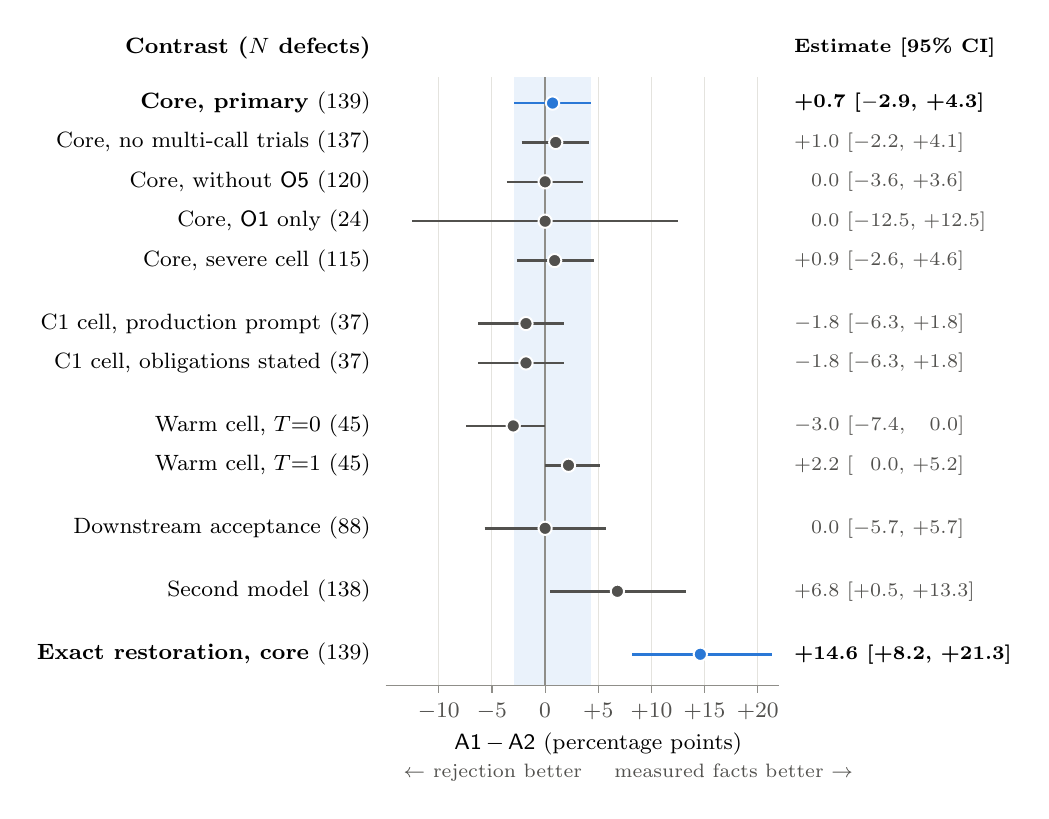
\begin{tikzpicture}[x=0.135cm, y=-0.5cm, font=\footnotesize]
  \definecolor{fpaccent}{HTML}{2A78D6}
  \definecolor{fpink}{HTML}{52514E}
  \definecolor{fpgrid}{HTML}{E4E3DE}
  \definecolor{fpzero}{HTML}{8F8E89}

  % \fprow{y}{label}{lo}{est}{hi}{text}{colour}
  \newcommand{\fprow}[7]{%
    \node[anchor=east, align=right] at (-15.5,#1) {#2};
    \draw[#7, line width=0.9pt] (#3,#1) -- (#5,#1);
    \filldraw[fill=#7, draw=white, line width=0.7pt] (#4,#1) circle (2.4pt);
    \node[anchor=west, text=fpink, font=\scriptsize] at (22.5,#1) {#6};
  }

  % last data row (exact restoration) sits at y = 15.0
  \def\ybottom{15.8}

  % primary interval band
  \fill[fpaccent!10] (-2.9,0.35) rectangle (4.3,\ybottom);
  % gridlines and zero line (solid hairlines)
  \foreach \gx in {-10,-5,5,10,15,20}
    \draw[fpgrid, line width=0.35pt] (\gx,0.35) -- (\gx,\ybottom);
  \draw[fpzero, line width=0.5pt] (0,0.35) -- (0,\ybottom);

  % column heads
  \node[anchor=east, font=\footnotesize\bfseries] at (-15.5,-0.4)
       {Contrast ($N$ defects)};
  \node[anchor=west, font=\scriptsize\bfseries] at (22.5,-0.4)
       {Estimate [95\% CI]};

  % --- core (confirmatory, then pre-specified companions)
  \fprow{1}{\textbf{Core, primary} (139)}{-2.9}{0.7}{4.3}%
        {\textcolor{black}{\textbf{+0.7 [$-$2.9, +4.3]}}}{fpaccent}
  \fprow{2}{Core, no multi-call trials (137)}{-2.2}{1.0}{4.1}%
        {+1.0 [$-$2.2, +4.1]}{fpink}
  \fprow{3}{Core, without \op{O5} (120)}{-3.6}{0.0}{3.6}%
        {\phantom{+}0.0 [$-$3.6, +3.6]}{fpink}
  \fprow{4}{Core, \op{O1} only (24)}{-12.5}{0.0}{12.5}%
        {\phantom{+}0.0 [$-$12.5, +12.5]}{fpink}
  \fprow{5}{Core, severe cell (115)}{-2.6}{0.9}{4.6}%
        {+0.9 [$-$2.6, +4.6]}{fpink}
  % --- constraint disclosure
  \fprow{6.6}{C1 cell, production prompt (37)}{-6.3}{-1.8}{1.8}%
        {$-$1.8 [$-$6.3, +1.8]}{fpink}
  \fprow{7.6}{C1 cell, obligations stated (37)}{-6.3}{-1.8}{1.8}%
        {$-$1.8 [$-$6.3, +1.8]}{fpink}
  % --- warm resampling
  \fprow{9.2}{Warm cell, $T{=}0$ (45)}{-7.4}{-3.0}{0.0}%
        {$-$3.0 [$-$7.4, \phantom{+}0.0]}{fpink}
  \fprow{10.2}{Warm cell, $T{=}1$ (45)}{0.0}{2.2}{5.2}%
        {+2.2 [\phantom{$-$}0.0, +5.2]}{fpink}
  % --- pipeline level
  \fprow{11.8}{Downstream acceptance (88)}{-5.7}{0.0}{5.7}%
        {\phantom{+}0.0 [$-$5.7, +5.7]}{fpink}
  % --- second model (Qwen2.5-7B-Instruct, local)
  \fprow{13.4}{Second model (138)}{0.5}{6.8}{13.3}%
        {+6.8 [+0.5, +13.3]}{fpink}
  % --- exact restoration (exploratory mechanism)
  \fprow{15.0}{\textbf{Exact restoration, core} (139)}{8.2}{14.6}{21.3}%
        {\textcolor{black}{\textbf{+14.6 [+8.2, +21.3]}}}{fpaccent}

  % x axis
  \draw[fpzero, line width=0.4pt] (-15,\ybottom) -- (22,\ybottom);
  \foreach \gx/\lab in {-10/$-$10,-5/$-$5,0/0,5/+5,10/+10,15/+15,20/+20} {
    \draw[fpzero, line width=0.4pt] (\gx,\ybottom) -- (\gx,\ybottom+0.18);
    \node[anchor=north, text=fpink] at (\gx,\ybottom+0.2) {\lab};
  }
  \node[anchor=north] at (5,\ybottom+0.95)
       {\arm{A1}\,$-$\,\arm{A2} (percentage points)};
  \node[anchor=north east, text=fpink, font=\scriptsize] at (4.4,\ybottom+1.75)
       {$\leftarrow$ rejection better};
  \node[anchor=north west, text=fpink, font=\scriptsize] at (5.6,\ybottom+1.75)
       {measured facts better $\rightarrow$};
\end{tikzpicture}

\caption{Selected \arm{A1}\,$-$\,\arm{A2} contrasts, with 95\%
bootstrap intervals over defects. The shaded band is the primary interval. Rows
below the first are exploratory or secondary. The penultimate row is the second
model (Section~\ref{sec:results-rq6}); the bottom row is the exploratory
exact-restoration contrast (Section~\ref{sec:results-rq2}).}
\label{fig:forest}
\end{figure*}

% ---------------------------------------------------------------------
\subsection{Pre-recorded predictions and input size}
\label{sec:results-predictions}
Repair exceeded the pre-recorded predictions for both feedback arms, and the
predicted class ordering reversed: referential defects were hardest. An
exploratory review-count analysis found lower repair or exact restoration at
the largest input stratum for some reasoning operators. The small strata and
nonmonotonic patterns do not establish an input-size mechanism; detailed
predictions, operator-specific rates and slopes are in Appendix~\ref{app:diagnostics}.

% ---------------------------------------------------------------------
\subsection{RQ2: Exact restoration and artifact presentation}
\label{sec:results-rq2}

Many repaired outputs restore the clean output. We define \emph{exact restoration} once for the entire paper as
canonical-JSON identity to the clean pre-injection stage output (parsed JSON
serialised with sorted keys and invariant whitespace). Under this definition,
100\% of trials that achieve exact restoration are verified as \cls{repaired}
(706 of 706 across all \cell{T2} arms, 337 of 337 in \cell{T2L}, and 319 of
319 in \cell{T2W}).

\paragraph{Unconditional exact restoration contrast}
Taking exact restoration as an unconditional outcome over all trials yields a
causally clean arm contrast within matched defects. On the core (\cell{T2},
$N=139$ paired defects), measured facts substantially increase exact
restoration: \arm{A1} restores 68.1\% of defects and \arm{A2} 53.5\%, an
advantage of \textbf{+14.6\pp{} \ci{+8.2}{+21.3}} (exact McNemar $p=0.00132$,
26 \arm{A1}-only vs 7 \arm{A2}-only discordant defects). At the trial level,
288 of 421 \arm{A1} retries (68.4\%) reproduce the clean output as canonical JSON,
compared to 223 of 417 (53.5\%) for \arm{A2}, 149 of 209 (71.3\%) for \arm{A0},
and 46 of 102 (45.1\%) for \arm{A3}.

The exploratory restoration contrast was positive in both warm-cell temperatures; effort-level results vary and are reported in Section~\ref{sec:results-thinking}.
In the warm-resampling cell (\cell{T2W}, $N=45$), \arm{A1} leads \arm{A2} by
\textbf{+20.7\pp{} \ci{+8.1}{+34.1}} at $T=0$ (69.6\% vs 48.9\%, $p=0.021$)
and by \textbf{+20.0\pp{} \ci{+8.9}{+32.6}} at $T=1$ (68.9\% vs 48.9\%,
$p=0.0039$). On the second
model (\cell{T2L}, Qwen2.5-7B, $N=138$), pooled exact restoration is lower and the
overall gap is narrow: \arm{A1} 42.0\% vs \arm{A2} 39.4\% (+2.7\pp{} \ci{-4.6}{+9.9},
$p=0.572$, 16 vs 12 discordant).

\paragraph{Trial-level decomposition}
The decomposition in Appendix~\ref{app:diagnostics} separates exact copies,
repaired rewrites, replacements or deletions, and outputs where the check
still fires. On the local model, the latter occurred in 32/414 \arm{A1} and
107/413 \arm{A2} trials. These outcome categories do not reveal whether the
model located the defect. Within-rewrite comparisons condition on a
post-treatment outcome and are descriptive.

\paragraph{Evidence consistent with copy-and-correct}
At temperature~0, canonical-JSON identity alone cannot separate two mechanisms. The model
might copy the artifact it is shown and fix the one injected change, or it
might re-derive its original answer from the same prompt. The warm-resampling
cell provides evidence bearing on them (Table~\ref{tab:mechanism}). At \arm{P1}, where the
artifact is shown, canonical-JSON identity to the clean output does not move with
temperature: \arm{A1} 69.6\% at $T=0$ and 68.9\% at $T=1$; \arm{A2} 48.9\% at
both. \arm{A3}, which sees no artifact, falls from 45\% identical as canonical JSON in the
core to \textbf{0\%} at $T=1$. A fresh draw at $T=1$ never reproduces the clean
output. An \arm{A1} retry shown the defective output reproduces it about two
times in three, at either temperature. This pattern is consistent with copying and correcting the shown artifact, although it does not identify the model's internal process. Repair stays at the ceiling at $T=1$
(\arm{A1} 99.3\%, \arm{A2} 97.0\%), so the null is not an artefact of greedy
decoding. Neither reading fixed in advance for this cell applies: canonical-JSON identity
did not fall, and neither did repair.

The cell also gives a budget-accounted comparison that
\citet{olausson2024selfrepair} require. \arm{A1}'s single retry at $T=0$ repairs
97.0\% at about 9.7k tokens per trial. \arm{A3}'s best-of-$k$ at $T=1$, taking
repetitions in execution order, reaches 82.2\%, 88.9\% and 93.3\% for $k=1,2,3$,
at about 13.6k tokens per draw (41k for $k=3$). In this setting, one retry with
the artifact in view repairs at least as often as three fresh draws (97.0\%
against 93.3\%), at under a quarter of their token cost. The
\arm{A1}\,$-$\,\arm{A2} gap is $-3.0$\pp{} \ci{-7.4}{0.0} at $T=0$ and
$+2.2$\pp{} \ci{0.0}{+5.2} at $T=1$. Their difference, $+5.2$\pp{}
\ci{+0.7}{+11.1}, is one of many exploratory intervals in this paper and rests
on a handful of defects. We do not read it as evidence that content matters
under sampling.

Repetitions at $T=0$ are nearly identical. Of the \arm{A1} cells
(defect\,$\times$\,arm) with all three repetitions, 73\% produce one distinct
output and 27\% produce two. The figures are 60\% and 40\% for \arm{A2}, where
one cell of 139 gave three distinct outputs, and 77\% and 23\% for \arm{A0}.
The exception is \arm{A3} at \arm{P0}, where 94\% of cells give two distinct
outputs.

\begin{table*}[t]
\centering
\caption{What moves repair (RQ2). Every row is \arm{A1} at \arm{P1} and
$T=0$ unless stated. Each cell re-runs its comparators in-session. Rates are
per-defect means with 95\% intervals over defects. Canonical-JSON identity is per
trial.}
\label{tab:mechanism}
\footnotesize
\begin{tabularx}{\linewidth}{@{}Y r L{2.7cm} L{3.6cm}@{}}
\toprule
Cell and level & $N$ & Repaired [95\% CI] & Contrast [95\% CI] \\
\midrule
\multicolumn{4}{@{}l}{\emph{Placement}} \\
\quad \arm{P0} artifact absent (production) & 45 & 94.1 \ci{88.1}{98.5} &
  \arm{P1}\,$-$\,\arm{P0} +3.7 \ci{-1.5}{+9.6} \\
\quad \arm{P1} artifact under review & 45 & 97.8 \ci{94.1}{100} &
  \arm{P1}\,$-$\,\arm{P2} 0.0 \ci{-4.4}{+4.4} \\
\quad \arm{P2} artifact as own turn & 45 & 97.8 \ci{93.3}{100} &
  \arm{P3}\,$-$\,\arm{P2} $-0.7$ \ci{-2.2}{0.0} \\
\quad \arm{P3} own turn + marker & 45 & 97.0 \ci{91.1}{100} &
  \arm{P1}\,$-$\,\arm{P3} +0.7 \ci{-2.2}{+4.4} \\
\multicolumn{4}{@{}l}{\emph{Temperature (warm cell)}} \\
\quad \arm{A1}, $T=1$ & 45 & 99.3 \ci{97.8}{100} & identity 68.9\% (69.6\% at
  $T=0$) \\
\quad \arm{A2}, $T=1$ & 45 & 97.0 \ci{94.1}{99.3} & identity 48.9\% (48.9\% at
  $T=0$) \\
\quad \arm{A3} at \arm{P0}, $T=1$ & 45 & 80.7 \ci{71.9}{88.9} & identity 0\%
  (45\% at $T=0$, core) \\
\multicolumn{4}{@{}l}{\emph{\op{O1} severity}} \\
\quad level 1: one id corrupted & 24 & 86.1 \ci{72.2}{97.2} & 1\,$-$\,2:
  $-2.8$ \ci{-11.1}{+5.6} \\
\quad level 2: every id of the pattern & 24 & 88.9 \ci{76.4}{98.6} & \\
\multicolumn{4}{@{}l}{\emph{Constraint disclosure (gap = \arm{A1}\,$-$\,\arm{A2})}} \\
\quad C0, production prompt & 37 & \arm{A1} 94.6, \arm{A2} 96.4 & gap $-1.8$
  \ci{-6.3}{+1.8} \\
\quad C1, obligations restated & 37 & \arm{A1} 92.8, \arm{A2} 94.6 & gap $-1.8$
  \ci{-6.3}{+1.8} \\
\quad difference of gaps & 37 & & 0.0 \ci{-6.3}{+6.3} \\
\bottomrule
\end{tabularx}
\end{table*}

\paragraph{Placement}
With the artifact in view, the observed framing contrasts were small. \arm{P1}, \arm{P2} and
\arm{P3} repair at 97.0--97.8\%, and the paired contrasts among them are within
a defect or two of zero. The pre-recorded prediction
\arm{P1}\,$\gg$\,\arm{P2} does not hold. A self-attribution effect of the kind
reported by \citet{tsui2026scbench} and \citet{chen2026rolerelabel} cannot
appear at a ceiling. \arm{P0}, the production placement, repairs 94.1\%, which
is not detectably lower than \arm{P1} ($+3.7$\pp{} \ci{-1.5}{+9.6}). It differs
in two other ways. First, \arm{P0} retries damage the rest of the output:
collateral damage is \textbf{38.4\%} of measurable trials at \arm{P0}, against
1.1\% at \arm{P1} and 3.4\% at \arm{P2} and \arm{P3}. A model that cannot see
its output regenerates everything, and the regeneration churns items that were
correct. Second, every one of the 16 report-stage defects needed a
schema-correction second call at \arm{P0}, and 50 of the cell's 52 multi-call
trials were at \arm{P0}. Without its multi-call trials, \arm{P0} repairs 90.8\%
\ci{81.6}{97.7} of the remaining 29 defects.

\paragraph{Severity and constraint disclosure}
Breaking all of a pattern's evidence did not lower repair. Level~2 of \op{O1}
repaired 88.9\%, against 86.1\% at level~1 ($-2.8$\pp{} \ci{-11.1}{+5.6}).
Restating the stage's obligations at retry time yielded no detectable difference in this small cell. The
\arm{A1}\,$-$\,\arm{A2} gap was $-1.8$\pp{} under both C0 and C1, and the
difference of gaps was 0.0\pp{} \ci{-6.3}{+6.3}, as pre-recorded. This imprecise comparison does not rule out an effect of disclosure.

\paragraph{Serving drift}
Every exploratory cell re-ran its comparators in-session, so each re-run is a
test--retest measurement of the hosted model at temperature~0, days after the
core. Against the core's trials for the same defect, arm and repetition, the
re-runs reproduced the outcome class in 95.8--99.6\% of pairs, across the four
cells that re-ran a core condition. They reproduced the output byte for byte in
only 76.4--83.3\% of pairs. For the C1 cell, 213 of 222 pairs (96\%) kept their
class and 185 (83\%) were byte-identical. Temperature~0 on a hosted API is
reproducible in outcome, not in output. A comparison across sessions would have
mixed that drift into every contrast. A local runtime was steadier, but not
bit-identical either (Section~\ref{sec:results-rq6}).

% ---------------------------------------------------------------------
\subsection{RQ3: Real defects are not injected defects}
\label{sec:results-rq3}

\begin{table*}[t]
\centering
\caption{The production retry on real, production-caught defects (13 defects in
7 business\,$\times$\,stage cells; arms at \arm{P0}; $r=3$). ``Accepted'' means
the supervisor routes the retried output to no retry. Intervals resample cells.
Descriptive only.}
\label{tab:tier1}
\footnotesize
\begin{tabularx}{\linewidth}{@{}Y r r r@{}}
\toprule
& \arm{A1} (production) & \arm{A2} & \arm{A3} \\
\midrule
Accepted & 28.2 \ci{15.1}{46.2} & 76.9 \ci{55.6}{89.7} & 25.6 \ci{12.8}{41.7}
  \\
Originally fired checks resolved & 38.5 & 76.9 & 33.3 \\
Returned the original defective output & 0.0 & 0.0 & 48.7 \\
Trace class (8 defects): production check accepts & 29.2 & 79.2 & 29.2 \\
Trace class: content-word check accepts & 87.5 & 100.0 & 79.2 \\
\midrule
\multicolumn{4}{@{}l}{\emph{Same criterion, injected defects at \arm{P0}}} \\
Accepted, injected (placement and core cells) & 98.5 & -- & 98.0 \\
\bottomrule
\end{tabularx}
\end{table*}

The 13 real defects are those the production supervisor caught in the 28
observe-mode runs. Replaying them through the production retry (\arm{A1} at
\arm{P0}) gives a very different picture from the injected defects
(Table~\ref{tab:tier1}). The supervisor accepted the retried output for
\textbf{28.2\%} of real defects. On the same criterion, at the same placement,
it accepted \arm{A1} retries for \textbf{98.5\%} of injected defects and
\arm{A3} regenerations for 98.0\% (25.6\% on real defects). By stage, injected
reasoning defects were accepted at 100\% against 26.7\% for real ones; at the
strategy stage the figures were 88.9\% and 29.2\%. All 13 real defects fire a check class targeted by an operator; the injected report-containment class has no real-bank counterpart. Coupling at the level of the check class therefore did not
make the injected defects representative of repair.

The reason is visible in what the real defects are. The pre-study audit
(Section~\ref{sec:design-operators}) found none of the 11 audited production-caught
defects to be errors. Nine were
checker false positives with a diagnosed cause: six paraphrases that the
character-level trace matcher failed to recognise, and three single-character
identifier corruptions where the real evidence was present. The calibration of
Section~\ref{sec:results-calibration} measures the trace matcher's
false-positive rate on grounded content at 5.0\%. A retry cannot fix a defect
that is not there. When the regenerated output again paraphrases its upstream,
the same check rejects it again. On the trace class, the content-word check
that the study's scorer uses accepts 87.5\% of \arm{A1} retries, while the
production check accepts 29.2\%.

One pattern runs against the RQ1 result and should be stated rather than
smoothed. On real defects, the contentless rejection (\arm{A2}) was accepted far
more often than the production feedback (76.9\% against 28.2\%), in both
stages. A plausible reading is that naming the flagged item invites the model
to rewrite that item specifically, and it rewrites it again in words the
lexical matcher does not credit. But 13 defects in seven cells support no
inference, and the cell was pre-registered as descriptive. We report it as a
hypothesis for a larger bank of real defects. \arm{A3} returned the original
defective output in 48.7\% of trials. \arm{A1} and \arm{A2} never did.

% ---------------------------------------------------------------------
\subsection{RQ4: Repair does not become pipeline-level improvement}
\label{sec:results-rq4}

\begin{table*}[t]
\centering
\caption{Downstream propagation (90 defects with a later stage). Later stages
are re-run once each, in observe mode, from each starting point. E1: every later
stage accepted. E2: the planted \op{O5} issue appears in the final report
(20 \op{O5} defects). E3: share of the clean run's final-report claims missing
from the condition's report. ``Noise floor'' is a second clean run. Means, and
paired contrasts with 95\% intervals over defects. Usable \arm{A1}/\arm{A2} starting points comprise 70/69 reasoning and 19/19 strategy defects (89/88 total). E2 uses 20 unrepaired and 19 per retry arm.}
\label{tab:downstream}
\footnotesize
\begin{tabularx}{\linewidth}{@{}Y r r r r r@{}}
\toprule
& Clean & Noise floor & Unrepaired & \arm{A1} & \arm{A2} \\
\midrule
E1 accepted & 84.4 & -- & 80.0 & 88.8 & 88.6 \\
E2 planted issue in report & 0 & -- & \textbf{70} & 0 & 0 \\
E3 divergence from clean & -- & 2.6 & \textbf{10.8} & 6.7 & 7.4 \\
\midrule
\multicolumn{6}{@{}l}{\emph{Paired contrasts}} \\
\quad E1: unrepaired\,$-$\,clean & \multicolumn{5}{l}{$-4.4$ \ci{-14.4}{+6.7}} \\
\quad E1: \arm{A1}\,$-$\,unrepaired & \multicolumn{5}{l}{$+7.9$ \ci{-1.1}{+16.9}} \\
\quad E1: \arm{A1}\,$-$\,\arm{A2} & \multicolumn{5}{l}{$\phantom{+}0.0$ \ci{-5.7}{+5.7}} \\
\quad E3: unrepaired\,$-$\,noise floor & \multicolumn{5}{l}{$+8.2$ \ci{+5.6}{+11.0}} \\
\quad E3: \arm{A1}\,$-$\,noise floor & \multicolumn{5}{l}{$+4.1$ \ci{+1.4}{+6.8}} \\
\quad E3: \arm{A1}\,$-$\,unrepaired & \multicolumn{5}{l}{$-4.2$ \ci{-7.5}{-1.0}} \\
\quad E3: \arm{A1}\,$-$\,\arm{A2} & \multicolumn{5}{l}{$-0.6$ \ci{-3.5}{+2.3}} \\
\bottomrule
\end{tabularx}
\end{table*}

Table~\ref{tab:downstream} follows each defect into the later stages. Of the
three readings fixed before the pass, the first holds and the second holds in
part.

\paragraph{Defects propagate silently}
Pipelines carrying an \emph{unrepaired} defect were accepted by every
downstream check about as often as clean ones ($-4.4$\pp{} \ci{-14.4}{+6.7}).
Yet their final reports diverged from the clean report by 8.2\pp{} beyond the
noise floor \ci{+5.6}{+11.0}. For \op{O5}, 70\% of unrepaired runs carried the
planted, untraceable recommendation into the final report. Once a later stage
has built on a defect, the later stages' own checks do not see it.

\paragraph{Downstream outcomes after retry}
The planted issue appeared in 14/20 unrepaired reports and 0/19 reports in
each retry arm. Across all \arm{A1}-started conditions, including failed
repairs, divergence was 4.2\,pp \ci{-7.5}{-1.0} below unrepaired conditions
but 4.1\,pp \ci{+1.4}{+6.8} above the noise floor. The overall arm contrast
was 0.0\,pp on E1 and $-0.6$\,pp \ci{-3.5}{+2.3} on E3; neither establishes
a difference between arms.

\paragraph{Downstream divergence by restoration outcome}
Table~\ref{tab:downstream-split} describes post-treatment subgroups. For
reasoning defects, reports following \arm{A1} exact copies diverged 4.16\%
against their matched 2.60\% noise floor; repaired rewrites diverged 16.65\%
against their matched 3.90\% floor. The corresponding excesses for \arm{A2}
were +1.30 and +8.61\,pp. Strategy rewrites had much smaller excesses
(+0.64 and 0.00\,pp). These are observational associations, not evidence that
copying caused preservation: the groups differ after treatment and matching
noise floors does not remove selection bias. The overall arm contrast on E3
was $-0.6$\,pp \ci{-3.5}{+2.3}.

\begin{table*}[t]
\centering
\caption{Downstream report divergence (E3) partitioned by observed upstream retry outcome (RQ4).
Each upstream condition is classified as \cls{repaired\_copy}, \cls{repaired\_rewrite},
or \cls{fail} against its pre-injection clean stage output. Divergence is the share of
clean final-report claims missing; ``Noise floor'' is an in-session second clean run for
the identical defects.}
\label{tab:downstream-split}
\footnotesize
\begingroup
\setlength{\tabcolsep}{3pt}
\begin{tabular*}{\linewidth}{@{\extracolsep{\fill}}l c r rrr c rrr@{}}
\toprule
& & & \multicolumn{3}{c}{\textbf{Arm \arm{A1} (Measured Facts)}} & & \multicolumn{3}{c}{\textbf{Arm \arm{A2} (Rejection)}} \\
\cmidrule(lr){4-6} \cmidrule(lr){8-10}
Subgroup & Upstream Group & $n$ & E3 (\%) & Noise (\%) & Excess & $n$ & E3 (\%) & Noise (\%) & Excess \\
\midrule
\multirow{3}{*}{\textbf{All defects ($N=90$)}} 
  & \cls{repaired\_copy}    & 50 & 3.82 & 2.40 & \textbf{+1.43\pp} & 37 & 2.60 & 1.44 & \textbf{+1.16\pp} \\
  & \cls{repaired\_rewrite} & 31 & 9.94 & 2.27 & \textbf{+7.67\pp} & 42 & 10.20 & 4.05 & \textbf{+6.15\pp} \\
  & \cls{fail}             &  8 & 11.90 & 5.06 & \textbf{+6.85\pp} &  9 & 14.07 & 0.79 & \textbf{+13.28\pp} \\
\midrule
\multirow{3}{*}{\shortstack[l]{\textbf{Reasoning stage}\\\textbf{(\op{O1}--\op{O3}, $N=70$)}}} 
  & \cls{repaired\_copy}    & 46 (65.7\%) & 4.16 & 2.60 & \textbf{+1.55\pp} & 33 (47.8\%) & 2.91 & 1.62 & \textbf{+1.30\pp} \\
  & \cls{repaired\_rewrite} & 18 (25.7\%) & 16.65 & 3.90 & \textbf{+12.75\pp} & 30 (43.5\%) & 14.28 & 5.67 & \textbf{+8.61\pp} \\
  & \cls{fail}             &  6 (8.6\%)  & 13.10 & 6.75 & \textbf{+6.35\pp} &  6 (8.7\%)  & 15.95 & 1.19 & \textbf{+14.76\pp} \\
\midrule
\multirow{3}{*}{\shortstack[l]{\textbf{Strategy stage}\\\textbf{(\op{O5}, $N=20$)}}} 
  & \cls{repaired\_copy}    &  4 & 0.00 & 0.00 & \textbf{0.00\pp} &  4 & 0.00 & 0.00 & \textbf{0.00\pp} \\
  & \cls{repaired\_rewrite} & 13 & 0.64 & 0.00 & \textbf{+0.64\pp} & 12 & 0.00 & 0.00 & \textbf{0.00\pp} \\
  & \cls{fail}             &  2 & 8.33 & 0.00 & \textbf{+8.33\pp} &  3 & 10.32 & 0.00 & \textbf{+10.32\pp} \\
\bottomrule
\end{tabular*}
\endgroup
\end{table*}

\paragraph{The report check rewards propagation}
The 20 unrepaired \op{O5} runs split cleanly. All 14 whose report carried the
planted issue were accepted. All 6 whose report did \emph{not} carry it were
rejected by the report-containment check. That check verifies that the report
restates its upstream. When the upstream is defective, a faithful report
passes and a report that departs from the defect fails. The check measures
fidelity to upstream, not correctness.

\paragraph{Defect-level and pipeline-level outcomes are loosely coupled}
All 8 \arm{A1} runs whose defect the core had \emph{not} repaired passed every
downstream check. Of the 81 runs whose defect was repaired, 10 did not. This is
the loose coupling between failure-mode presence and task outcome that
\citet{cemri2025mast} report for multi-agent traces. Clean pipelines themselves
failed the supervisor in 15.6\% of runs (76 of 90 accepted). Across both clean repetitions, 29 of 180 conditions were rejected at the strategy traceability check.

\paragraph{Calibrated verifier acceptance}
Offline re-scoring of all 447 downstream conditions under the calibrated
content-word traceability check (\code{Jaccard}~$\ge 0.10$ replacing character-level
\code{difflib}~$\ge 0.35$ on strategy outputs) shows how acceptance changes under the alternative matcher; acceptance is not a correctness measure. Clean pipeline acceptance (E1) jumps from
\textbf{84.4\%} (76 of 90) to \textbf{96.7\%} (87 of 90): three strategy traceability flags remained under the content-word matcher; their semantic validity was not independently established.
Accepted runs under \arm{A1} rise from \textbf{88.8\%} (79 of 89) to
\textbf{97.8\%} (87 of 89), and under \arm{A2} from \textbf{88.6\%} (78 of 88)
to \textbf{98.9\%} (87 of 88). Unrepaired pipeline acceptance rises from
\textbf{80.0\%} to \textbf{93.3\%} (84 of 90; the 6 rejected runs are precisely
the 6 \op{O5} runs where the final report dropped the planted ungrounded recommendation).

% ---------------------------------------------------------------------
\subsection{RQ5: Overwrite is a cost decision, not a correctness decision}
\label{sec:results-rq5}

Routed to a retry instead of overwritten, a divergent frequency was repaired in
\textbf{69 of 69} \arm{A1} trials, for 23 of 23 defects (exact 95\% interval
over defects \ci{85.2}{100}). No trial showed collateral damage. A fresh
regeneration (\arm{A3}) repaired 97.1\% \ci{92.8}{100}, with collateral damage
in 30.4\% of trials. The overwrite is exact by construction and costs no model
call. The retry costs one call and about 22k tokens. By the reading fixed before
the freeze, the overwrite was a \emph{cost} decision, not a correctness one. The
design principle it exemplifies (any quantity the checker can compute should
not be asked of the model) rests on that zero-call argument and on exactness,
not on any failure of the retry.

% ---------------------------------------------------------------------
\subsection{Calibration of the checks}
\label{sec:results-calibration}

Two checks can be calibrated without model calls.

\paragraph{The frequency check}
The frequency check behaves exactly as specified. Sweeping \op{O4}'s divergence
over 23 bases, detection is 0\% for every divergence up to 0.04 and 100\% from
0.051. At exactly 0.05 it is 52.2\%, because the check is a strict $>0.05$ and
floating-point rounding of the injected value splits those 23 cases 12 to 11.

\paragraph{The traceability check}
The traceability check is imprecise in both directions. On the 139
recommendation issues of every clean strategy output in the 28 runs, all of
them grounded by construction, the production character-level matcher fires on
\textbf{5.0\%}: the 7 issues whose best lexical similarity to their own
upstream falls below 0.35. The content-word matcher fires on none. On 150
foreign issues placed on other businesses, the production matcher fires on
96.0\% and the content-word matcher on 100\%. The production matcher both
flags grounded paraphrase and misses foreign content. This is the measured
cause of the real-defect results in Section~\ref{sec:results-rq3}, and of the
clean-run rejections in Section~\ref{sec:results-rq4}.

A further observation concerns the pipeline, not repair. Run from its
production prompt, the report stage needed a schema-correction second call
every time: in all 447 downstream conditions, and for all 16 report-stage
defects at \arm{P0}.

% ---------------------------------------------------------------------
\subsection{RQ6: A second model}
\label{sec:results-rq6}
% Source: backend/out_study/T2L/analysis.json (repair_analysis.py --cell c7);
% gates: C7_preflight_r3/gates.json (G2 carried over from C7_preflight/);
% verification: T2L/verification.json. Exploratory throughout (A10, A11).

The second-model cell asks whether the core's answers belong to the method or
to the hosted model. Qwen2.5-7B-Instruct retried the same injected defects,
built on the hosted model's clean outputs, under the core's arms
(Section~\ref{sec:design-cells}). All of it is exploratory. G1 passed. G3
excluded four defects before any call (\op{O1} and \op{O2} on two businesses
whose reasoning prompts, at 31{,}504--31{,}916 tokens, exceeded the 28{,}608
left after the output reserve), leaving 138. G2 failed, with 8 of 10 pairs
identical, which led to A11; G4 passed, with 8 of 10 first calls valid. All
930 trials ran, 929 were usable, and every offline score agreed with its live
score.

\begin{table*}[t]
\centering
\caption{The second model (RQ6; exploratory): Qwen2.5-7B-Instruct retrying
the hosted model's injected defects at \arm{P1}, $r=3$. Rates are per-defect
means; intervals are 95\% bootstrap intervals over defects; $p$ is the exact
McNemar test on the majority dichotomy, reported descriptively.
``Identical'' compares a retried output with the clean output as canonical
JSON, the comparison behind the hosted model's identity shares.}
\label{tab:rq6}
\footnotesize
\begin{tabularx}{\linewidth}{@{}Y r r r l r@{}}
\toprule
Contrast & $N$ & \arm{A1} & \arm{A2} & Difference [95\% CI] & $p$ \\
\midrule
\textbf{All eligible defects} & \textbf{138} & \textbf{72.9} & \textbf{66.2} &
  \textbf{+6.8 \ci{+0.5}{+13.3}} & \textbf{0.052} \\
\quad first repetition only & 137 & 73.0 & 67.2 & +5.8 \ci{-0.7}{+12.4} &
  0.134 \\
\quad \op{O1} only (production-like) & 22 & 39.4 & 47.0 & $-7.6$
  \ci{-25.8}{+10.6} & 1.000 \\
\quad severe cell only (\op{O2}--\op{O7}) & 116 & 79.3 & 69.8 & +9.5
  \ci{+3.2}{+16.4} & 0.013 \\
\quad reasoning stage & 66 & 58.6 & 42.9 & & \\
\quad strategy stage & 20 & 75.0 & 80.0 & & \\
\quad report stage & 52 & 90.4 & 90.4 & & \\
\quad hosted model, same defects$^a$ & 137 & 96.8 & 95.6 & & \\
\midrule
\multicolumn{6}{@{}l}{\emph{Shares of trials (\arm{A1} 414, \arm{A2} 413) and
  of cells, \%}} \\
\quad \cls{unrepaired}: check still fires & & 7.7 & 25.9 & & \\
\quad \cls{replaced}: another passing value & & 15.7 & 6.5 & & \\
\quad identical to the clean output & & 42.0 & 39.5 & & \\
\quad collateral damage$^b$ & & 10.5 & 15.2 & & \\
\quad cells with identical raw text$^c$ & & 94.9 & 84.7 & & \\
\bottomrule
\end{tabularx}

\smallskip
\parbox{\linewidth}{\footnotesize $^a$ 137 defects for \arm{A1} and 135 for
\arm{A2}. $^b$ Of the 258 and 257 trials where it is measurable. $^c$ Of the
138 and 137 defect\,$\times$\,arm cells with three usable repetitions, those
whose raw outputs were identical in every call of all three.}
\end{table*}

\paragraph{The contrast, below the ceiling}
Both arms repaired well below the hosted model's ceiling
(Table~\ref{tab:rq6}): \textbf{72.9\%} \ci{65.5}{80.2} under measured facts and
\textbf{66.2\%} \ci{58.2}{73.9} under the rejection, a difference of
\textbf{+6.8\pp{} \ci{+0.5}{+13.3}}. The discordant defects split 16 to 6, and
the exact McNemar test gives $p=0.052$. The first repetition alone gives
+5.8\pp{} \ci{-0.7}{+12.4}, and counting the lost trial as unrepaired changes
nothing. Two of the four readings fixed in advance apply. The contrast was
measured with headroom, unlike the core's, and its interval excludes zero,
which is exploratory evidence that measured facts help this model. The
borderline test and the first-repetition interval keep that evidence a
hypothesis. The gap sits in the severe cell and at the reasoning stage, and it
is largest for fabricated identifiers (\op{O2}) and mislabelled aspects
(\op{O3}). The report stage tied, and on \op{O1}, as on the hosted model,
measured facts gained nothing.

\paragraph{How the arms fail}
After a contentless rejection the injected check still fired in \textbf{107 of
413} retries; after measured facts, in 32 of 414. Told only that its output
was wrong, the model often left the defect where it was. Told what was wrong,
it acted on the named item, though 65 times it changed it to another value that
passed the check (27 under the rejection). The hosted model left the check
firing in only 3 and 2 retries.

\paragraph{Copying, stability and regeneration}
Copy-and-correct carries over at a lower rate: 42.0\% and 39.5\% of retries
reproduced the clean output exactly, against 68\% and 53\% on the hosted model,
and still more than half of each arm's repairs did. Collateral damage was
higher, at 10.5\% and 15.2\% against 1.5\% and 0.4\%. The local runtime was
steadier than the hosted API but not bit-reproducible: across three
back-to-back repetitions, 94.9\% of \arm{A1} cells and 84.7\% of \arm{A2} cells
returned identical raw text, a stricter test than the comparison of parsed
outputs behind the hosted model's 73\%. \arm{A3}'s 38.2\% \ci{20.6}{55.9} is
not interpretable here. Every trial is scored against the hosted model's clean
output, which \arm{A1} and \arm{A2} can see and restore but a fresh draw from
another model cannot reproduce. \arm{A3} repaired no reasoning defect. Its
repairs come from the report stage, where removing an inserted item is the
repair, and all 36 of those trials needed a schema-correction call; without
them \arm{A3} repaired 4.5\%.

\paragraph{Against the hosted model}
Paired on the same defects, the second model's repair rate differed from the
hosted model's by $-24.1$\pp{} \ci{-32.4}{-16.1} under measured facts and
$-29.4$\pp{} \ci{-37.5}{-21.5} under the rejection. Family, size, quantisation and
runtime all differ, and the bases are the hosted model's. The comparison
places the ceiling in the hosted model without saying which difference
produces it.

% ---------------------------------------------------------------------
\subsection{Thinking-budget sweep (\cell{T2T})}
\label{sec:results-thinking}
% Source: backend/out_study/T2T/analysis.json (repair_analysis.py --cell thinking);
% verification: T2T/checkpoint.jsonl. Exploratory throughout (A12).

An exploratory sweep asks how configured thinking budget relates to repair and restoration.
Under Amendment~A12 (\cell{T2T}), we executed a prospective within-weights sweep
varying \texttt{reasoning\_effort} across four levels (\texttt{none}, \texttt{low},
\texttt{medium}, \texttt{high}) on \model{}, covering 45 defects ($N=45$, matching
the stratified 1/3 stride of \cell{T2P} and \cell{T2W}) with three repetitions
(1{,}224 trials, 100\% usable, 100\% offline score agreement, consuming 11.16M tokens).
Arms \arm{A1} and \arm{A2} ran at \arm{P1} on all 45 defects (540 trials per arm),
while the regeneration baseline \arm{A3} ran at \arm{P0} on 12 defects (144 trials).
Table~\ref{tab:thinking} compiles the empirical results.

\begin{table*}[t]
\centering
\caption{Within-weights thinking-budget sweep (\cell{T2T}).
Sweeping \texttt{reasoning\_effort} across four levels on \model{} ($N=45$ defects, $r=3$, 1{,}224 trials).
Rates and exact restoration $P(\text{exact copy})$ are defect-level means with 95\% cluster-bootstrap CIs.
The within-weights regeneration baseline \arm{A3}@\arm{P0} runs on $N=12$ defects (36 trials/level).
Multi-attempt counts denote trials requiring schema retry ($>1$ call).}
\label{tab:thinking}
\footnotesize
\begingroup
\setlength{\tabcolsep}{2pt}
\begin{tabular*}{\linewidth}{@{\extracolsep{\fill}}l r r c c r c c r c r r@{}}
\toprule
& Budget & Thinking tokens / & \multicolumn{3}{c}{\textbf{Binary Repair Rate (\%)}} & \multicolumn{3}{c}{\textbf{Exact Restoration $P(\text{copy})$ (\%)}} & \arm{A3}@\arm{P0} & \multicolumn{2}{c}{\textbf{Multi-Attempt}} \\
\cmidrule(lr){4-6} \cmidrule(lr){7-9} \cmidrule(lr){11-12}
Effort & Cap & Trial & \arm{A1} & \arm{A2} & Diff [95\% CI] & \arm{A1} & \arm{A2} & Diff [95\% CI] & Repair [95\% CI] & \arm{A1} & \arm{A2} \\
\midrule
\texttt{high} & 24{,}576 & 2{,}682 & 97.8 & 100.0 & $-2.2$ \ci{-6.7}{0.0} & 60.7 & 50.4 & +10.4 \ci{-3.0}{+23.0} & 75.0 \ci{50.0}{100.0} & 0 & 0 \\
\texttt{medium} & 8{,}192 & 2{,}557 & 94.8 & 94.8 & \phantom{+}0.0 \ci{-7.4}{+7.4} & 60.0 & 51.1 & +8.9 \ci{-2.2}{+20.0} & 88.9 \ci{72.2}{100.0} & 0 & 5 \\
\texttt{low} & 1{,}024 & 914 & 99.3 & 98.5 & +0.7 \ci{0.0}{+2.2} & 59.3 & 35.6 & \textbf{+23.7 \ci{+11.9}{+36.3}}$^{**}$ & 80.6 \ci{58.3}{100.0} & 0 & 4 \\
\texttt{none} & 0 & 0 & 100.0 & 100.0 & \phantom{+}0.0 \ci{0.0}{0.0} & 80.7 & 57.0 & \textbf{+23.7 \ci{+12.6}{+36.3}}$^{***}$ & \textbf{91.7 \ci{75.0}{100.0}} & 7 & 21 \\
\bottomrule
\end{tabular*}
\endgroup

\smallskip
\parbox{\linewidth}{\footnotesize $p$-values from exact McNemar tests on discordant defect majorities: all binary repair contrasts have $p=1.000$; for exact restoration, $p=0.302$ (\texttt{high}), $p=0.754$ (\texttt{medium}), $^{**}p=0.007$ (\texttt{low}), and $^{***}p=0.001$ (\texttt{none}).}
\end{table*}

At \texttt{none}, all 135 trials in each feedback arm were scored repaired.
This demonstrates the observed performance with a zero thinking-token budget,
not a single forward pass: seven \arm{A1} and 21 \arm{A2} trials required
schema-correction calls, compared with none at \texttt{high}. Mean \arm{A1}
latency was 7.17 seconds at \texttt{none} versus 17.44 seconds at \texttt{high}.
The exact-restoration contrast varied nonmonotonically across levels, reaching
+23.7\,pp \ci{+12.6}{+36.3} at \texttt{none}; the exploratory effort-step
slope was +5.48\,pp \ci{+0.44}{+10.59}, whereas the log-budget slope interval
included zero. \arm{A3} repair also varied nonmonotonically (75.0\%, 88.9\%,
80.6\%, 91.7\% from high to none). These results do not identify internal
reasoning mechanisms.

% =====================================================================
\section{Discussion}
\label{sec:discussion}
% =====================================================================

\subsection{What the feedback buys, and what it does not}
\label{sec:discussion-content}

The confirmatory result is a null, and a ceiling bounds what it can mean.
Measured-fact feedback and a contentless rejection repaired injected defects
equally well, to within about 4 percentage points. Both sat near the capability
ceiling, which \arm{A0} reached in every trial. For defects of this kind, on
this model, it does not matter what the supervisor says, provided the model is
told that something is wrong and can see what it produced. Restating the
stage's obligations at retry time did not matter either. That excludes the
explanation \citet{huang2024cannot} and \citet{kamoi2024} warn of, in which
measured feedback wins by teaching the task. The C1 gap and the C0 gap were
identical.

The mechanism suggests why. We offer it as an interpretation, not a tested
claim. Derivability works in both directions. The supervisor can detect an
injected defect because the defect is inconsistent with upstream state that the
pipeline holds. That same upstream state is in the retried stage's prompt. An
evidence identifier that matches none of the reviews the stage was given, or a
recommendation unrelated to any pattern it was given, is as visible to a capable
model holding its own output and its inputs as it is to the checker. The
measured fact repeats what the model can already see. On this reading the
copy-and-correct pattern is to be expected: the model keeps what is consistent
with its inputs and reverts what is not, and the result is often its original
output byte for byte.

The result therefore sides with the accounts that locate the active ingredient
in the signal and in what the model can see
\citep{chen2024selfdebug,chen2026rolerelabel,tsui2026scbench}. It does not side
with those that locate it in feedback content~\citep{olausson2024selfrepair},
but only for defects this easy to undo. The core says nothing about defects the
model cannot see or cannot fix. The one cell with headroom, the
production-like \op{O1} at 84.7\%, gives the same answer: \arm{A1} and \arm{A2}
were identical. Its interval of $\pm12.5$\pp{} is too wide to exclude a
moderate effect.

The second model supplies the headroom that the core lacks, and there a gap
opens: measured facts led by +6.8\pp{} \ci{+0.5}{+13.3}, mostly at the
reasoning stage (Section~\ref{sec:results-rq6}). The gap is exploratory and
fragile ($p=0.052$, and the first repetition alone includes zero), but its form
fits the mechanism above. Without the measured fact, the second model left the
defect in place after a quarter of its retries; with it, after fewer than one
in ten. The fact supplied the location of the inconsistency, which the hosted
model found unaided. Models that cannot find their reasoning errors can
correct many of them once told where they are~\citep{tyen2024}, and the second
model behaved that way. Location is not always enough: on \op{O1}, where the
fix is to recover an exact identifier, naming it helped neither model. On this
evidence the null is a property of a capable model at its ceiling, not of the
method. We read the gap as a hypothesis: feedback content matters to the
extent that the model cannot find the defect by itself.

\subsection{Placement is the design lever the production retry lacks}
\label{sec:discussion-placement}

The production retry does not show the model its rejected output; it runs at
\arm{P0}. Showing the output (\arm{P1}) left repair statistically unchanged
($+3.7$\pp{} \ci{-1.5}{+9.6}). It cut collateral damage from 38.4\% of retries
to 1.1\%, and it avoided a schema-correction call that every report-stage retry
at \arm{P0} needed. A model that cannot see its output regenerates all of it,
and regeneration churns content that was correct. The same comparison favours
showing the artifact at equal budget. One retry at \arm{P1} repaired 97.0\%
of defects, at about a quarter of the token cost of three fresh draws, which
repaired 93.3\%. These results are exploratory and come from one model. But they
point to a change that costs nothing to make and is invisible to every
repair-rate metric: return the rejected output with the rejection. The second
model did not test placement, and below the ceiling wording mattered too
(Section~\ref{sec:discussion-content}). But the production feedback already
carries the measured facts; showing the output is the change that remains.

\subsection{A supervisor's precision bounds the value of its retries}
\label{sec:discussion-precision}

On real, production-caught defects the production retry was accepted 28.2\% of
the time. The obvious reading is that real defects are harder to fix. The data
support a different one. Most real defects were checker false positives: the
pre-study audit found none of them to be an error to a human rater, and the
calibration measured the trace check firing on 5.0\% of grounded
recommendations. The retry cannot repair content that is already correct. It
regenerates the content in other words, and the same lexical check rejects it
again. The rate also shows in clean runs: 16\% of clean pipelines in the
downstream pass were rejected, every one by the trace check. A false positive
costs a model call, and at the retry cap it becomes a halt or a warning on a
run that had nothing wrong with it. For the engineer of such a supervisor, the
precision of each check matters more than the wording of the feedback. On our
data, a content-word matcher fired on no grounded issue and on every foreign
one. We kept the production supervisor unchanged, because it is the system
under study. Replacing its matcher is the obvious follow-up, and we have not
evaluated it.

The same result is a caution for fault-injection studies of LLM systems in
general. The injected defects coupled to the real ones at the level of check
class: every real defect fires a class that some operator targets. Their repair
rates were nonetheless 98.5\% and 28.2\%. For this system, the question
\citet{just2014mutants} raised for program repair has a negative answer.
A repair rate measured on injected defects is not an estimate of the rate on
the defects the system produces, and coupling by class does not make it one. A
study that reports only injected-defect repair should not describe it as a
production repair rate. Ours does not, and the replay is what entitles us to
say so.

\subsection{Local checks verify fidelity, not correctness}
\label{sec:discussion-local}

An unrepaired defect passed the downstream checks about as often as a clean
run, and the report-containment check \emph{rewarded} carrying it forward. The
reason is structural. A check that verifies each stage against its upstream
certifies consistency, and consistency with a defective upstream is still
consistency. Once a defect has been accepted where it arose, every later check
treats it as ground truth. This is a property of derivability-based
verification in general, not of our thresholds. The conference
version~\citep{hoang2026eas} noted that ``an accepted claim may inherit an
upstream error''; the downstream pass measures it. Two consequences follow.
First, such a supervisor needs its recall at the point of origin, because
downstream checks cannot make up for a miss
upstream. Second, repair is not restoration. Repaired runs removed the planted
content but still diverged from the clean report beyond the noise floor,
because a repaired stage is a regenerated stage. Together with the loose
coupling between defect-level and pipeline-level outcomes, this is the pattern
\citet{cemri2025mast} report for multi-agent failures. A supervisor that
improves the defect-level rate need not move the run-level outcome, and
evaluations should report both.

\subsection{What the overwrite bought}
\label{sec:discussion-overwrite}

The retry repaired every divergent frequency it was given, without collateral
damage. The recompute-and-overwrite design was therefore not needed for
correctness. It is still the better design, for reasons the counterfactual makes
precise: it is exact by construction, costs no call, cannot introduce churn, and
does not depend on the model's cooperation. The principle that a quantity the
checker can compute should not be asked of the model stands. It stands on cost
and determinism, not on any failure of the alternative.

\subsection{Revisions to the conference version}
\label{sec:discussion-reconcile}

The new results qualify four claims of~\citet{hoang2026eas}.
\begin{enumerate}
\item \emph{``At temperature zero an unchanged prompt returns an unchanged
  answer, so the content of that feedback, not the act of retrying, is what can
  change the outcome.''}
  Both halves need qualifying. On a hosted API, temperature~0 reproduced a
  trial's outcome class across sessions in 96\% to over 99\% of pairs, but its
  output byte for byte in only 76--83\%. Within a single session, 27\% of \arm{A1}
  cells still produced two distinct outputs across three repetitions. A local
  runtime serving one request at a time did better, but two of ten prompts sent
  twice still returned different text. And with the artifact in view, the
  content of the feedback did not change the outcome on the hosted model. On the
  second model it changed it modestly (Section~\ref{sec:results-rq6}).
\item \emph{Defect incidence (35\% of runs) and instability (20\%).} These
  rates count the supervisor's verdicts. Some of those verdicts are false
  positives of the trace check, which fires on 5.0\% of grounded
  recommendations. Some identifier flags are single-character corruptions where
  the real evidence is present. The rates should be read as rates of supervisor
  flags. The rate of genuinely ungrounded content is lower by an amount this
  study bounds but does not measure.
\item \emph{Recompute-and-overwrite} was asserted as a principle with no
  counterfactual. It is now measured: it was a cost decision, not a correctness
  decision (Section~\ref{sec:results-rq5}).
\item \emph{Retry repair} was unmeasured, because the enforcing arm produced one
  retry. The hosted model repairs injected defects at the ceiling under any
  feedback; the second model repairs 66--73\% of them. The
  real defects the supervisor caught are accepted after the production retry
  28.2\% of the time, for the reasons in
  Section~\ref{sec:discussion-precision}.
\end{enumerate}
% Author decision 3 (JOURNAL_PAPER_PLAN.md section 2), closed 2026-10-23:
% items 2 and 4 are journal findings, following the precedent set for the
% matcher defect on 2026-09-14, not a note to the conference chairs. If the
% FISAT camera-ready changes any of the four claims quoted above, revise this
% list to match the published version.

\subsection{Recommendations for building runtime supervisors}
\label{sec:discussion-recommendations}

Five practical lessons follow for engineers who put a deterministic checker in
the control path of an LLM pipeline. All are scoped to one pipeline. Lessons
1, 3 and 4 rest on the hosted model alone. The second model qualifies lesson 2
and extends lesson 5 to a local runtime.
\begin{enumerate}
\item \textbf{Return the rejected output with the rejection.} Repair stayed the
  same, collateral damage fell from 38\% to 1\%, and one retry repaired at
  least as often as three fresh draws, at under a quarter of their token cost.
\item \textbf{Invest in check precision before feedback wording.} Wording made
  no measurable difference on the hosted model. On the second model, naming
  the defect helped by an exploratory 6.8 points, apparently by showing the
  model where the defect was. Keep the measured facts, which cost nothing, but do not
  expect them to make up for an imprecise check. False positives made up most
  of what the production retry was asked to fix.
\item \textbf{Verify where defects arise.} Stage-local consistency checks
  certify fidelity to upstream, so they cannot catch a defect after a later
  stage has built on it.
\item \textbf{Compute what can be computed.} Overwriting a derivable statistic
  is exact, free and churn-free. A retry achieves the same correctness at a
  cost.
\item \textbf{Treat temperature~0 as non-deterministic, on a hosted API and on
  a local runtime alike, and check injected defects against real ones.} Match
  every comparison within a serving session. Replay real defects before reading
  an injected-defect repair rate as a production one.
\end{enumerate}

% =====================================================================
\section{Threats to validity}
\label{sec:threats}
% Sources: PREREGISTRATION.md section 9; JOURNAL_PLAN.md D14-D16 and section
% 15; RESULTS.md section 8.
% =====================================================================

\paragraph{Construct validity}
The main threat is the ceiling. The injected defects were easy for this model
to undo, so RQ1 measures the effect of feedback content on defects that the
model repairs regardless. It says nothing about defects the model cannot see
or fix. The severity sweep did not create headroom, and the one cell with
headroom (\op{O1}) is small. The second model has headroom, and there a modest
gap appears (Section~\ref{sec:results-rq6}), so the confirmatory null is a
result about a model at its ceiling. That cell scores every trial against the
hosted model's clean output, which \arm{A1} and \arm{A2} can restore but
\arm{A3}'s fresh draws cannot; \arm{A3} is not interpreted there. The
construct is repair \emph{by regeneration}, and
the outcome is the replacement value. That is stricter than the supervisor's
own check, which a different but resolving identifier would satisfy. \arm{A1}
is both specific and correct, and no arm offers specific but wrong feedback.
The claim is therefore about feedback content, not about specificity as such.
Recommendation issues are generic enough that no string matcher separates a
restored issue cleanly from a different one: under the scorer, a different
restaurant's recommendation ``restores'' 41\% of the time. This is why the
primary contrast is also reported without \op{O5}, where it is unchanged.
Collateral damage is measured only for item classes with a calibrated churn
floor, so report-stage trials are excluded from it. On real defects, the
outcome is acceptance by the supervisor's own checks, which are imprecise. We
report the content-word reading beside it, and we do not call either reading
repair.

\paragraph{Internal validity}
Hosted-model drift is the threat this design spends most on. All arms of a
defect run in one session, no contrast crosses sessions, and every exploratory
cell re-runs its comparators in-session. The re-runs measure the drift; they do
not assume it away. One interim look at outcome counts, for budget, is
disclosed. Amendments A5--A12 were filed after earlier results were known. All
are exploratory, their designs follow a grid fixed before any result, and each
pass's readings were fixed before it ran. The second-model cell's determinism
gate failed, and A11 changed that cell's design before any final trial; the
failure is reported, not relabelled. The warm cell (A7) and thinking sweep (A12)
were designed in response to the core's pattern and are reported as tests of
those explanations.
The analysis code postdates the core. It transcribes rules fixed at the freeze,
was tested on synthetic rows first, and every live score was reproduced
offline. Trials that needed a schema-correction second call carry a turn of the
model's own output. They are analysed separately, and the primary estimate does
not move without them. The core's trial losses come from the network and from
the client machine sleeping; their relationship to arm cannot be ruled out solely by session matching. The second model's
one loss came from its context guard, and counting it as unrepaired changes
nothing. Finally, the authors
built both the supervisor and the operators. The validity gates guarantee that
each operator trips the check it targets and no other, and blinded raters
judged injected defects against real ones. Neither guarantees that the
operators resemble what the model produces, and Section~\ref{sec:results-rq3}
shows that they do not.

Copy versus rewrite is a post-treatment outcome; within-group comparisons may reflect selection and are descriptive.

\paragraph{External validity}
The confirmatory trials used one model, served by one provider at
temperature~0 (temperature~1 in the warm cell), with a single retry. One
exploratory cell repeated the core's arms on a 7.6-billion-parameter
open-weight model from another family, served locally. Report-stage rates tied on that model; \op{O1} did not show an advantage for \arm{A1}.
The hosted-model ceiling did not carry over, and below it measured facts gained an exploratory 6.8
points. Placement, the real-defect replay, propagation, and the thinking sweep
rest on the hosted model alone. Two models are not a population: family, size,
quantisation and runtime change together between these two, and the second
model retried defects in the first model's outputs instead of running its own
pipeline. The study covers one pipeline in one domain, with 28 workloads
stratified by input size, and the pipeline is closed by design. The derivability
property that makes its supervision deterministic does not hold for agents that
retrieve, call tools or carry memory across runs~\citep{hoang2026eas}. The
results transfer to such systems only in their parts that remain closed. The
seven operators that ran cover five check classes. The real-defect bank is 13
defects in 7 cells, most of them one class.

\paragraph{Conclusion validity}
There is one confirmatory test: the primary RQ1 overall repair contrast
(+0.7\pp{} \ci{-2.9}{+4.3}, $p=0.754$). It was powered at 0.875 for a 12-point
effect, and its null is reported as an interval, not as an absence of evidence.
Near a ceiling, few defects can be discordant, which limits what any test of this
contrast could show. That is why the estimate, not the test, is primary.
Everything else is exploratory, with no correction for multiplicity. Exact
restoration and downstream subgroup analyses were discovered post hoc; the
thinking sweep was designed after the core result and does not independently
confirm a mechanism. Copy and rewrite are post-treatment outcomes, so their
association with downstream divergence is subject to selection bias. Any other single
interval that excludes zero, such as the warm cell's difference of gaps, \arm{A2}'s
advantage on real defects or the second model's +6.8 points, should be read as a
hypothesis, not a finding. The second model's case is weaker still: its exact test
does not reject ($p=0.052$), and its first repetition alone gives an interval that
includes zero. The real-defect cell supports no test at all. Bootstrap intervals for
rates at 100\% degenerate to a point, so exact intervals over defects are
reported where a rate is at the boundary.

% =====================================================================
\section{Conclusion}
\label{sec:conclusion}
% =====================================================================

We asked whether the measured facts a deterministic supervisor writes into a
retry prompt are what repairs a defective stage in an LLM pipeline. The
pre-registered answer is no, for injected defects. A rejection that said
nothing repaired them as well as one that named the offending item and its
measured value: the difference was +0.7 percentage points, with an interval
that excludes anything larger than about 4. The reason is that the model,
shown its defective output, mostly copies it back and corrects the one
inconsistency it can see. The information the supervisor measures is in the
model's context too. A second model that repaired far less often gained an
exploratory 6.8 points from the measured facts, apparently because they told it
where the defect was; the null describes a capable model, not every model.

What the supervisor \emph{does} matters more than what it \emph{says}. Showing
the model its rejected output left repair unchanged and cut collateral damage
by an order of magnitude. The precision of a check decides whether a retry
fixes anything: on the defects the supervisor really caught in production, most
of them its own false positives, the production retry was accepted 28\% of the
time. Stage-local checks certify consistency with upstream, so a defect that
gets past its own stage is invisible to every later stage and is sometimes
rewarded by them. And a statistic the supervisor can compute is better
overwritten than retried. A retry also fixes it, but only an overwrite does so
exactly and at no cost.

For engineers, the lesson is to spend effort on where a check looks and how
precisely it fires, not on how its complaint is worded beyond naming what
failed. For researchers who
evaluate LLM systems by fault injection, the lesson is one that mutation
testing learned for detection: injected faults stand in for real ones only once
a coupling study shows that they do. Until then, a repair rate measured on
injected defects is a property of the operators. It is not yet evidence about
the defects the system actually produces.


\nolinenumbers
% =====================================================================
%  End matter required by JSS (Guide for Authors, read 2026-10-08):
%  CRediT statement, competing interests, funding, data statement, and the
%  generative-AI declaration "in a new section before the references list".
%  Every block below is a DRAFT for the authors to confirm or rewrite.
% =====================================================================

\section*{CRediT authorship contribution statement}
\TODO{Author list is open (decision D5). Assign CRediT roles per author:
Conceptualization, Methodology, Software, Validation, Formal analysis,
Investigation, Data curation, Writing -- original draft, Writing -- review \&
editing, Visualization, Supervision, Project administration.}

\section*{Declaration of competing interest}
The authors declare that they have no known competing financial interests or
personal relationships that could have appeared to influence the work reported
in this paper. \TODO{confirm for every author}

\section*{Funding}
This research did not receive any specific grant from funding agencies in the
public, commercial, or not-for-profit sectors. \TODO{confirm; state who paid
for the model API usage if that counts as funding}

\section*{Data availability}
\TODO{Author decision 4 (JOURNAL\_PAPER\_PLAN.md section 2). Draft follows;
fill in the repository URL and an archived DOI (e.g.\ Zenodo). Check the Yelp
Open Dataset terms before redistributing stage outputs derived from reviews.
JSS applies research-data Option~C (deposit and cite, or explain), and its Open
Science Initiative reviews availability after acceptance -- consider opting in.}
The pre-registration (frozen at the annotated tag \code{prereg-freeze}), the
pipeline and supervisor, the injection and analysis code, every trial record and
every analysis output are available at [repository URL, archived as DOI]. Each
number in this paper is regenerated from the committed trial records by the
committed analysis scripts, without model calls. The Yelp Open Dataset is
available from its provider under its own terms~\citep{yelpdataset}.

\section*{Declaration of generative AI and AI-assisted technologies in the manuscript preparation process}
\TODO{Required by Elsevier whenever AI tools were used. The authors must state
the actual scope; this draft was produced with Claude Code, and earlier
sessions used it for study code and analysis. Rewrite to match what happened.}
During the preparation of this work the authors used Claude (Anthropic), through
the Claude Code tool, in order to draft and revise the manuscript text, tables
and LaTeX source from the study's committed records, and to assist in writing
and testing the study's software and analysis scripts. After using this tool,
the authors reviewed and edited the content as needed and take full
responsibility for the content of the published article.

\section*{Acknowledgements}
\TODO{Thank the two raters of the blinded defect audit if they are not authors,
and anyone else who helped.}


\bibliographystyle{elsarticle-harv}
\bibliography{references}

\appendix
% =====================================================================
\section{Arm and placement wording}
\label{app:wording}
% Verbatim from backend/scripts/arms.py (AUTHORED_WORDING, frozen 2026-08-25;
% C1 wording added by prereg amendment A1, 2026-09-20) and from
% backend/app/agents/base_agent.py (_SUPERVISOR_FEEDBACK_PROMPT, the
% production template). Print them with:  python scripts/arms.py
% =====================================================================

Every trial starts from the production prompt of the stage being re-run: its
system and user turns, exactly as production builds them. Arms and placements
only \emph{append} turns. Table~\ref{tab:messages} gives the turns each cell
appends, in order, and the wording follows. \code{\{output\}} is the defective
stage output as JSON. \code{\{feedback\}} is the supervisor's measured fact
(Section~\ref{sec:system-feedback}).

\begin{table}[htbp]
\centering
\caption{Turns appended to the production stage prompt, per arm and placement.
``--'' marks the two structurally undefined cells.}
\label{tab:messages}
\footnotesize
\begin{tabularx}{\linewidth}{@{}l Y Y Y@{}}
\toprule
& \arm{P0} & \arm{P1} & \arm{P2} (\arm{P3}) \\
\midrule
\arm{A0} & -- & user: A0 preamble + output & user: A0 preamble; assistant:
  output (user: marker) \\
\arm{A1} & user: A1 feedback & user: framing + output; user: A1 feedback &
  assistant: output (user: marker); user: A1 feedback \\
\arm{A2} & user: A2 rejection & user: framing + output; user: A2 rejection &
  assistant: output (user: marker); user: A2 rejection \\
\arm{A3} & nothing & -- & -- \\
\bottomrule
\end{tabularx}
\end{table}

\paragraph{\arm{A1}: the production feedback template}
\begin{prompttext}
A deterministic quality check rejected your previous answer to this task:\\[2pt]
\{feedback\}\\[2pt]
Produce a corrected answer that fixes exactly these issues. Return only valid
JSON.
\end{prompttext}

\paragraph{\arm{A2}: the contentless rejection}
\begin{prompttext}
A deterministic quality check rejected your previous answer to this task.\\[2pt]
Produce a corrected answer. Return only valid JSON.
\end{prompttext}

\paragraph{\arm{A0}: the correction-task preamble}
\begin{prompttext}
Below is a draft answer to this task. Review it and produce the best answer you
can to the original task. Return only valid JSON.
\end{prompttext}

\paragraph{\arm{P1}: the framing of the artifact (arms \arm{A1}, \arm{A2})}
\begin{prompttext}
Your previous answer to this task was:\\[2pt]
\{output\}
\end{prompttext}

\paragraph{\arm{P3}: the correction marker}
\begin{prompttext}
The answer above contains an error.
\end{prompttext}

\paragraph{C1: the stage obligations restated at retry time}
Spliced into the stage prompt ahead of its closing output instruction; C0 is
the unmodified production prompt.
\begin{prompttext}
Your answer must satisfy all of the following requirements:
\end{prompttext}
followed by the obligations of the stage being retried:
\begin{description}[leftmargin=1.2em,style=nextline,font=\normalfont\itshape,
                   before=\footnotesize\raggedright]
\item[Reasoning] \texttt{- Every id in evidence\_review\_ids must be the
  review\_id of a review present in the analysed reviews you were given.}\\
  \texttt{- Every review cited as evidence for a pattern must itself mention
  that pattern's aspect.}
\item[Strategy] \texttt{- Every recommendation's issue must trace back to one of
  the reasoning patterns or root causes you were given.}
\item[Report] \texttt{- The report must only restate the upstream outputs you
  were given. Do not introduce a root cause or a recommendation that is not
  present upstream.}\\
  \texttt{- business\_name and sample\_size must match the values supplied with
  the task, not values inferred from the text.}
\end{description}
\noindent The frequency obligation is deliberately absent. That check resolves
to a warning, never to a retry, so it never reaches an \arm{A1} feedback string,
and stating it would give C1 information that \arm{A1} does not have.


\end{document}
